% !Mode:: "TeX:UTF-8"
\def\usewhat{dvipdfmx}                               % 定义编译方式 dvipdfmx 或者 pdflatex,默认为 dvipdfmx
                                                     % 方式编译,如果需要修改,只需改变花括号中的内容即可。
\documentclass[12pt,openany,oneside]{book}
                                                     % 本科生毕业论文通常采用单页排版
% !Mode:: "TeX:UTF-8"
%  Authors: 张井   Jing Zhang: prayever@gmail.com     天津大学2010级管理与经济学部信息管理与信息系统专业硕士生
%           余蓝涛 Lantao Yu: lantaoyu1991@gmail.com  天津大学2008级精密仪器与光电子工程学院测控技术与仪器专业本科生

%%%%%%%%%% Package %%%%%%%%%%%%
\usepackage{graphicx}                       % 支持插图处理
\usepackage[a4paper,text={150true mm,224true mm},top=35.5true mm,left=30true mm,head=5true mm,headsep=2.5true mm,foot=8.5true mm]{geometry}
                                            % 支持版面尺寸设置
\usepackage{titlesec}                       % 控制标题的宏包
\usepackage{titletoc}                       % 控制目录的宏包
\usepackage{fancyhdr}                       % fancyhdr宏包 支持页眉和页脚的相关定义
\usepackage[UTF8]{ctex}                     % 支持中文显示
\usepackage{color}                          % 支持彩色
\usepackage{amsmath}                        % AMSLaTeX宏包 用来排出更加漂亮的公式
\usepackage{amssymb}                        % 数学符号生成命令
\usepackage[below]{placeins}                %允许上一个section的浮动图形出现在下一个section的开始部分,还提供\FloatBarrier命令,使所有未处理的浮动图形立即被处理
\usepackage{flafter}                        % 使得所有浮动体不能被放置在其浮动环境之前,以免浮动体在引述它的文本之前出现.
\usepackage{multirow}                       % 使用Multirow宏包,使得表格可以合并多个row格
\usepackage{booktabs}                       % 表格,横的粗线;\specialrule{1pt}{0pt}{0pt}
\usepackage{longtable}                      % 支持跨页的表格。
\usepackage{tabularx}                       % 自动设置表格的列宽
\usepackage{subfigure}                      % 支持子图 %centerlast 设置最后一行是否居中
\usepackage[subfigure]{ccaption}            % 支持子图的中文标题
\usepackage[sort&compress,numbers]{natbib}  % 支持引用缩写的宏包
\usepackage{enumitem}                       % 使用enumitem宏包,改变列表项的格式
\usepackage{calc}                           % 长度可以用+ - * / 进行计算
\usepackage{txfonts}                        % 字体宏包
\usepackage{bm}                             % 处理数学公式中的黑斜体的宏包
\usepackage[amsmath,thmmarks,hyperref]{ntheorem}  % 定理类环境宏包,其中 amsmath 选项用来兼容 AMS LaTeX 的宏包
\usepackage{CJKnumb}                        % 提供将阿拉伯数字转换成中文数字的命令
\usepackage{indentfirst}                    % 首行缩进宏包
\usepackage{CJKutf8}                        % 用在UTF8编码环境下,它可以自动调用CJK,同时针对UTF8编码作了设置。
%\usepackage{hypbmsec}                      % 用来控制书签中标题显示内容

% 生成有书签的 pdf 及其生成方式。通常可以在 tjumain.tex 文件的第一行选择 pdflatex 或者是 dvipdfmx 编译手段。如果选择前者,则使用 pdflatex + pdflatex 编译; 如果选择后者,在编译的时候选择 latex + bibtex + latex + latex 编译。出现混淆的时候,系统会报错。

% 如果您的pdf制作中文书签有乱码使用如下命令,就可以解决了
\def\atemp{dvipdfmx}\ifx\atemp\usewhat
\usepackage[dvipdfmx,unicode,               % dvipdfmx 编译, 加入了中文复制,粘贴支持引擎。
            pdfstartview=FitH,
            bookmarksnumbered=true,
            bookmarksopen=true,
            colorlinks=false,
            pdfborder={0 0 1},
            citecolor=blue,
            linkcolor=red,
            anchorcolor=green,
            urlcolor=blue,
            breaklinks=true
            ]{hyperref}
\fi

\def\atemp{pdflatex}\ifx\atemp\usewhat
\usepackage{cmap}                            % pdflatex 编译时,可以生成可复制、粘贴的中文 PDF 文档, 缺点是在Windows上显示时效果不大好,字体发虚
\usepackage[pdftex,unicode,
            %CJKbookmarks=true,
            bookmarksnumbered=true,
            bookmarksopen=true,
            colorlinks=false,
            pdfborder={0 0 1},
            citecolor=blue,
            linkcolor=red,
            anchorcolor=green,
            urlcolor=blue,
            breaklinks=true
            ]{hyperref}
\fi

                                % 定义本文所使用宏包
\graphicspath{{figures/}}                            % 定义所有的 .eps 文件在 figures 子目录下
\begin{document}                                     % 开始全文
\begin{CJK*}{UTF8}{song}                             % 开始中文字体使用
% !Mode:: "TeX:UTF-8"
%  Authors: 张井   Jing Zhang: prayever@gmail.com     天津大学2010级管理与经济学部信息管理与信息系统专业硕士生
%           余蓝涛 Lantao Yu: lantaoyu1991@gmail.com  天津大学2008级精密仪器与光电子工程学院测控技术与仪器专业本科生

%%%%%%%%%%%%%%%%% Fonts Definition and Basics %%%%%%%%%%%%%%%%%
%\newcommand{\song}{\CJKfamily{song}}    % 宋体
%\newcommand{\fs}{\CJKfamily{fs}}        % 仿宋体
%\newcommand{\kai}{\CJKfamily{kai}}      % 楷体
%\newcommand{\hei}{\CJKfamily{hei}}      % 黑体
%\newcommand{\li}{\CJKfamily{li}}        % 隶书
\newcommand{\song}{\songti}    % 宋体
\newcommand{\fs}{\fangsong}        % 仿宋体
\newcommand{\kai}{\kaishu}      % 楷体
\newcommand{\hei}{\heiti}      % 黑体
\newcommand{\li}{\lishu}        % 隶书
\newcommand{\yihao}{\fontsize{26pt}{26pt}\selectfont}       % 一号, 单倍行距
\newcommand{\xiaoyi}{\fontsize{24pt}{24pt}\selectfont}      % 小一, 单倍行距
\newcommand{\erhao}{\fontsize{22pt}{1.25\baselineskip}\selectfont}       % 二号, 1.25倍行距
\newcommand{\xiaoer}{\fontsize{18pt}{18pt}\selectfont}      % 小二, 单倍行距
\newcommand{\sanhao}{\fontsize{16pt}{16pt}\selectfont}      % 三号, 单倍行距
\newcommand{\xiaosan}{\fontsize{15pt}{15pt}\selectfont}     % 小三, 单倍行距
\newcommand{\sihao}{\fontsize{14pt}{14pt}\selectfont}       % 四号, 单倍行距
\newcommand{\xiaosi}{\fontsize{12pt}{12pt}\selectfont}      % 小四, 单倍行距
\newcommand{\wuhao}{\fontsize{10.5pt}{10.5pt}\selectfont}   % 五号, 单倍行距
\newcommand{\xiaowu}{\fontsize{9pt}{9pt}\selectfont}        % 小五, 单倍行距

%\CJKtilde  % 重新定义了波浪符~的意义
% JUST DON'T USE CJK
% 使用 ctexbook 之后已无必要
\newcommand\prechaptername{第}
\newcommand\postchaptername{章}

\punctstyle{hangmobanjiao}             % 调整中文字符的表示,行内占一个字符宽度,行尾占半个字符宽度

% 调整罗列环境的布局
\setitemize{leftmargin=3em,itemsep=0em,partopsep=0em,parsep=0em,topsep=-0em}
\setenumerate{leftmargin=3em,itemsep=0em,partopsep=0em,parsep=0em,topsep=0em}

% 避免宏包 hyperref 和 arydshln 不兼容带来的目录链接失效的问题。
\def\temp{\relax}
\let\temp\addcontentsline
\gdef\addcontentsline{\phantomsection\temp}

% 自定义项目列表标签及格式 \begin{publist} 列表项 \end{publist}
\newcounter{pubctr} %自定义新计数器
\newenvironment{publist}{%%%%%定义新环境
\begin{list}{[\arabic{pubctr}]} %%标签格式
    {
     \usecounter{pubctr}
     \setlength{\leftmargin}{2.5em}   % 左边界 \leftmargin =\itemindent + \labelwidth + \labelsep
     \setlength{\itemindent}{0em}     % 标号缩进量
     \setlength{\labelsep}{1em}       % 标号和列表项之间的距离,默认0.5em
     \setlength{\rightmargin}{0em}    % 右边界
     \setlength{\topsep}{0ex}         % 列表到上下文的垂直距离
     \setlength{\parsep}{0ex}         % 段落间距
     \setlength{\itemsep}{0ex}        % 标签间距
     \setlength{\listparindent}{0pt}  % 段落缩进量
    }}
{\end{list}}

\makeatletter
\renewcommand\normalsize{
  \@setfontsize\normalsize{12pt}{12pt} % 小四对应 12 pt
  \setlength\abovedisplayskip{4pt}
  \setlength\abovedisplayshortskip{4pt}
  \setlength\belowdisplayskip{\abovedisplayskip}
  \setlength\belowdisplayshortskip{\abovedisplayshortskip}
  \let\@listi\@listI}
\def\defaultfont{\renewcommand{\baselinestretch}{1.63}\normalsize\selectfont} % 设置行距

\renewcommand{\CJKglue}{\hskip -0.1 pt plus 0.08\baselineskip} % 控制字间距,使每行 34 个汉字
\makeatother

%%%%%%%%%%%%% Contents %%%%%%%%%%%%%%%%%
\renewcommand{\contentsname}{目\qquad 录}
\setcounter{tocdepth}{2} % 控制目录深度
% 使用 ctexbook 之后已无必要
%\titlecontents{chapter}[2em]{\vspace{.5\baselineskip}\xiaosan\song}
             %{\prechaptername\CJKnumber{\thecontentslabel}\postchaptername\qquad}{}
             %{\hspace{.5em}\titlerule*[10pt]{$\cdot$}\sihao\contentspage}
\titlecontents{chapter}[2em]{\vspace{.5\baselineskip}\xiaosan\song}
             {\thecontentslabel\qquad}{}
             {\hspace{.5em}\titlerule*[10pt]{$\cdot$}\sihao\contentspage}
\titlecontents{section}[3em]{\vspace{.25\baselineskip}\sihao\song}
             {\thecontentslabel\quad}{}
             {\hspace{.5em}\titlerule*[10pt]{$\cdot$}\sihao\contentspage}
\titlecontents{subsection}[4em]{\vspace{.25\baselineskip}\sihao\song}
             {\thecontentslabel\quad}{}
             {\hspace{.5em}\titlerule*[10pt]{$\cdot$}\sihao\contentspage}

%%%%%%%%%% Chapter and Section %%%%%%%%%%%%%
\setcounter{secnumdepth}{4}
\setlength{\parindent}{2em}
\renewcommand{\chaptername}{\prechaptername\CJKnumber{\thechapter}\postchaptername}
\titleformat{\chapter}{\centering\xiaosan\song}{\hei\chaptername}{2em}{}
\titlespacing{\chapter}{0pt}{0.1\baselineskip}{0.8\baselineskip}
\titleformat{\section}{\sihao\hei}{\thesection}{1em}{}
\titlespacing{\section}{0pt}{0.15\baselineskip}{0.25\baselineskip}
\titleformat{\subsection}{\sihao\hei}{\thesubsection}{1em}{}
\titlespacing{\subsection}{0pt}{0.1\baselineskip}{0.3\baselineskip}
\titleformat{\subsubsection}{\sihao\hei}{\thesubsubsection}{1em}{}
\titlespacing{\subsubsection}{0pt}{0.05\baselineskip}{0.1\baselineskip}

%%%%%%%%%% Table, Figure and Equation %%%%%%%%%%%%%%%%%
\renewcommand{\tablename}{表}                                     % 插表题头
\renewcommand{\figurename}{图}                                    % 插图题头
\renewcommand{\thefigure}{\arabic{chapter}-\arabic{figure}}       % 使图编号为 7-1 的格式 %\protect{~}
\renewcommand{\thesubfigure}{\alph{subfigure})}                   % 使子图编号为 a) 的格式
\renewcommand{\thesubtable}{(\alph{subtable})}                    % 使子表编号为 (a) 的格式
\renewcommand{\thetable}{\arabic{chapter}-\arabic{table}}         % 使表编号为 7-1 的格式
\renewcommand{\theequation}{\arabic{chapter}-\arabic{equation}}   % 使公式编号为 7-1 的格式
\newcommand{\ud}{\mathrm{d}}

%%%%%% 定制浮动图形和表格标题样式 %%%%%%
\makeatletter
\long\def\@makecaption#1#2{
   \vskip\abovecaptionskip
   \sbox\@tempboxa{\centering\wuhao\song{#1\qquad #2} }
   \ifdim \wd\@tempboxa >\hsize
     \centering\wuhao\song{#1\qquad #2} \par
   \else
     \global \@minipagefalse
     \hb@xt@\hsize{\hfil\box\@tempboxa\hfil}
   \fi
   \vskip\belowcaptionskip}
\makeatother
\captiondelim{~~~~} %用来控制longtable表头分隔符

%%%%%%%%%% Theorem Environment %%%%%%%%%%%%%%%%%
\theoremstyle{plain}
\theorembodyfont{\song\rmfamily}
\theoremheaderfont{\hei\rmfamily}
\newtheorem{theorem}{定理~}[chapter]
\newtheorem{lemma}{引理~}[chapter]
\newtheorem{axiom}{公理~}[chapter]
\newtheorem{proposition}{命题~}[chapter]
\newtheorem{prop}{性质~}[chapter]
\newtheorem{corollary}{推论~}[chapter]
\newtheorem{definition}{定义~}[chapter]
\newtheorem{conjecture}{猜想~}[chapter]
\newtheorem{example}{例~}[chapter]
\newtheorem{remark}{注~}[chapter]
%\newtheorem{algorithm}{算法~}[chapter]
\newenvironment{proof}{\noindent{\hei 证明:}}{\hfill $ \square $ \vskip 4mm}
\theoremsymbol{$\square$}

%%%%%%%%%% Page: number, header and footer  %%%%%%%%%%%%%%%%%

%\frontmatter 或 \pagenumbering{roman}
%\mainmatter 或 \pagenumbering{arabic}
\makeatletter
\renewcommand\frontmatter{\clearpage
  \@mainmatterfalse
  }
\makeatother

%%%%%%%%%%% Code: Listings from MCM Template %%%%%%%%%%%%

\definecolor{grey}{rgb}{0.8,0.8,0.8}
\definecolor{darkgreen}{rgb}{0,0.3,0}
\definecolor{darkblue}{rgb}{0,0,0.3}
\def\lstbasicfont{\fontfamily{pcr}\selectfont\footnotesize}
\lstset{%
% indexing
   % numbers=left,
   % numberstyle=\small,%
% character display
    showstringspaces=false,
    showspaces=false,%
    tabsize=4,%
% style
    frame=lines,%
    basicstyle={\footnotesize\lstbasicfont},%
    keywordstyle=\color{darkblue}\bfseries,%
    identifierstyle=,%
    commentstyle=\color{darkgreen},%\itshape,%
    stringstyle=\color{black}%
}
\lstloadlanguages{C,C++,Java,Matlab,Mathematica,Python}

%%%%%%%%%%%% References %%%%%%%%%%%%%%%%%
\renewcommand{\bibname}{参考文献}
% 重定义参考文献样式,来自thu
\makeatletter
\renewenvironment{thebibliography}[1]{
    \titleformat{\chapter}{\raggedright\sihao\hei}{\chaptername}{2em}{}
   \chapter*{\bibname}
   \wuhao
   \list{\@biblabel{\@arabic\c@enumiv}}
        {\renewcommand{\makelabel}[1]{##1\hfill}
         \settowidth\labelwidth{0 cm}
         \setlength{\labelsep}{0pt}
         \setlength{\itemindent}{0pt}
         \setlength{\leftmargin}{\labelwidth+\labelsep}
         \addtolength{\itemsep}{-0.7em}
         \usecounter{enumiv}
         \let\p@enumiv\@empty
         \renewcommand\theenumiv{\@arabic\c@enumiv}}
    \sloppy\frenchspacing
    \clubpenalty4000
    \@clubpenalty \clubpenalty
    \widowpenalty4000
    \interlinepenalty4000
    \sfcode`\.\@m}
   {\def\@noitemerr
     {\@latex@warning{Empty `thebibliography' environment}}
    \endlist\frenchspacing}
\makeatother

\addtolength{\bibsep}{-0.5em}     % 缩小参考文献间的垂直间距
\setlength{\bibhang}{2em}         % 每个条目自第二行起缩进的距离

% 参考文献引用作为上标出现
%\newcommand{\citeup}[1]{\textsuperscript{\cite{#1}}}
\makeatletter
    \def\@cite#1#2{\textsuperscript{[{#1\if@tempswa , #2\fi}]}}
\makeatother
%% 引用格式
\bibpunct{[}{]}{,}{s}{}{,}

%%%%%%%%%%%% Cover %%%%%%%%%%%%%%%%%
% 封面、摘要、版权、致谢格式定义
\makeatletter
\def\ctitle#1{\def\@ctitle{#1}}\def\@ctitle{}
\def\cdegree#1{\def\@cdegree{#1}}\def\@cdegree{}
\def\caffil#1{\def\@caffil{#1}}\def\@caffil{}
\def\csubject#1{\def\@csubject{#1}}\def\@csubject{}
\def\cgrade#1{\def\@cgrade{#1}}\def\@cgrade{}
\def\cauthor#1{\def\@cauthor{#1}}\def\@cauthor{}
\def\cnumber#1{\def\@cnumber{#1}}\def\@cnumber{}
\def\csupervisor#1{\def\@csupervisor{#1}}\def\@csupervisor{}
\def\crank#1{\def\@crank{#1}}\def\@crank{}
\def\cdate#1{\def\@cdate{#1}}\def\@cdate{}
\long\def\cabstract#1{\long\def\@cabstract{#1}}\long\def\@cabstract{}
\long\def\eabstract#1{\long\def\@eabstract{#1}}\long\def\@eabstract{}
\def\ckeywords#1{\def\@ckeywords{#1}}\def\@ckeywords{}
\def\ekeywords#1{\def\@ekeywords{#1}}\def\@ekeywords{}
\def\cheading#1{\def\@cheading{#1}}\def\@cheading{}


\pagestyle{fancy}
  \fancyhf{}
  \fancyhead[C]{\song\wuhao \@cheading}  % 页眉显示天津大学 20XX 届本科生毕业论文
  \fancyfoot[C]{\song\xiaowu ~\thepage~}
\newlength{\@title@width}

% 定义封面
\def\makecover{
%\cleardoublepage%
   \phantomsection
    \pdfbookmark[-1]{\@ctitle}{ctitle}

    \begin{titlepage}
      \vspace*{31.5pt}
      \begin{center}

  \begin{figure}[h]
  \centering
  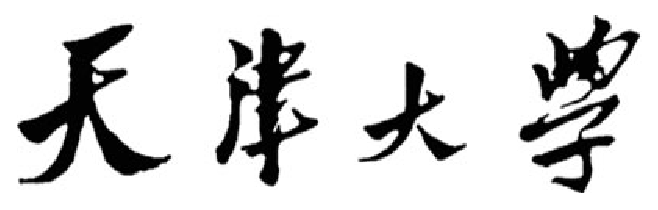
\includegraphics[width=0.4\textwidth]{figures/tju}
  \end{figure}
  \vspace*{21pt}
  \hei\erhao{\textbf{本科生毕业论文}}
  \vspace*{52.5pt}

  \begin{figure}[h]
  \centering
  
\includegraphics[width=0.3\textwidth]{figures/tjulogo.png}
  \end{figure}

  \vspace*{42pt}
  \renewcommand\arraystretch{1.5}
  \setlength{\@title@width}{5cm}
  {\sanhao\song{\bf{
  \begin{tabular}{lc}
    学\qquad 院&  \underline{\makebox[\@title@width][c]{\@caffil}} \\
    专\qquad 业 &  \underline{\makebox[\@title@width][c]{\@csubject}} \\
    年\qquad 级  &  \underline{\makebox[\@title@width][c]{\@cgrade}}\\
    姓\qquad 名 &  \underline{\makebox[\@title@width][c]{\@cauthor}} \\
    指导教师 &  \underline{\makebox[\@title@width][c]{\@csupervisor}} \\
  \end{tabular}}}
 }
  \vspace*{21pt}

\song\sanhao{\textbf{\@cdate}}
\end{center}
\end{titlepage}

%%%%%%%%%%%%%%%%%%%   Abstract and Keywords  %%%%%%%%%%%%%%%%%%%%%%%
\clearpage
\markboth{摘~要}{摘~要}
\pdfbookmark[0]{摘~~要}{cabstract}
%\addcontentsline{toc}{chapter}{摘~要}
%\chapter*{\centering\sanhao\hei\bfseries 摘\qquad 要}
\chapter*{\centering\sanhao\hei 摘\qquad 要}
\song\defaultfont
\@cabstract
\vspace{\baselineskip}

\hangafter=1\hangindent=52.3pt\noindent
{\hei\xiaosi 关键词:} \@ckeywords
\thispagestyle{empty}

%%%%%%%%%%%%%%%%%%%   English Abstract  %%%%%%%%%%%%%%%%%%%%%%%%%%%%%%
\clearpage
%\phantomsection
\markboth{ABSTRACT}{ABSTRACT}
\pdfbookmark[0]{ABSTRACT}{eabstract}
%\addcontentsline{toc}{chapter}{ABSTRACT}
\chapter*{\centering\sanhao{\bf{ABSTRACT}}}
%\vspace{\baselineskip}
\@eabstract
\vspace{\baselineskip}

\hangafter=1\hangindent=60pt\noindent
{\textbf{Keywords:}} \@ekeywords
\thispagestyle{empty}
}
\makeatother
                                 % 完成对论文各个部分格式的设置
\frontmatter                                         % 以下是论文导言部分,包括论文的封面,中英文摘要和中文目录
\fancypagestyle{plain}{
\fancyhf{}
\renewcommand{\headrulewidth}{0 pt}
\fancyfoot[C]{\song\xiaowu~\thepage~}
}
% !Mode:: "TeX:UTF-8"

%%  可通过增加或减少 setup/format.tex中的
%%  第274行 \setlength{\@title@width}{8cm}中 8cm 这个参数来 控制封面中下划线的长度。

\fancypagestyle{plain}{
\fancyhf{}
\renewcommand{\headrulewidth}{0 pt}
\fancyfoot[C]{\song\xiaowu~\thepage~}
}
\cheading{天津大学~2012~届本科生毕业设计}      % 设置正文的页眉,需要填上对应的毕业年份
\ctitle{天津大学本科生学位论文~\LaTeX~模板使用说明}    % 封面用论文标题,自己可手动断行
\caffil{精密仪器与光电子工程学院} % 学院名称
\csubject{测控技术与仪器}   % 专业名称
\cgrade{2008~级}            % 年级
\cauthor{余蓝涛}            % 学生姓名
\cnumber{3008202079}        % 学生学号
\csupervisor{宋~~乐}        % 导师姓名
\crank{讲~~师}              % 导师职称

%\cdate{\CTEXdigits{\the\year} 年\CJKnumber{\the\month} 月 \CJKnumber{\the\day} 日}  % 显示为中文日期格式
\cdate{\the\year~年~\the\month~月~\the\day~日}
\cabstract{
中文摘要一般在~400~字以内,简要介绍毕业论文的研究目的、方法、结果和结论,语言力求精炼。中英文摘要均要有关键词,一般为~3~—~7~个。字体为小四号宋体,各关键词之间要有分号。英文摘要应与中文摘要相对应,字体为小四号~Times New Roman,详见模板。
}

\ckeywords{关键词~1;关键词~2;关键词~3;……;关键词~7(关键词总共~3~—~7~个,最后一个关键词后面没有标点符号)}

\eabstract{
The upper bound of the number of Chinese characters is 400. The abstract aims at introducing the research purpose, research methods, research results, and research conclusion of graduation thesis, with refining words. Generally speaking, both the Chinese and English abstracts require the keywords, the number of which varies from 3 to 7, with a semicolon between adjacent words. The font of the English Abstract is Times New Roman, with the size of 12pt(small four).
}

\ekeywords{keyword 1, keyword 2, keyword 3, ……, keyword 7 (no punctuation at the end)}

\makecover

\clearpage
                                % 封面

%%%%%%%%%%   目录   %%%%%%%%%%
\defaultfont
\clearpage{\pagestyle{empty}\cleardoublepage}
\setcounter{page}{1}                                 % 单独从 1 开始编页码
\pagenumbering{arabic}
\titleformat{\chapter}{\centering\sanhao\hei}{\chaptername}{2em}{} % 设置目录两字的格式
\pdfbookmark[0]{目~~录}{mulu}
\tableofcontents                                     % 中文目录
\thispagestyle{plain}

\mainmatter\defaultfont\sloppy\raggedbottom
\makeatletter
\fancypagestyle{plain}{                              % 设置开章页眉页脚风格
    \fancyhf{}
    \fancyhead[C]{\song\wuhao \@cheading}            % 首页页眉格式
    \fancyfoot[C]{\song\xiaowu ~\thepage~}           % 首页页脚格式
    \renewcommand{\headrulewidth}{0.5pt}
    \renewcommand{\footrulewidth}{0pt}
}
\makeatother
\setcounter{page}{1}                                 % 单独从 1 开始编页码
\titleformat{\chapter}{\centering\xiaosan\hei}{\chaptername}{2em}{}
                                                     % 恢复chapter标题格式要求
% !Mode:: "TeX:UTF-8"

\chapter{模板介绍与注意事项}
\section{模板说明}

TJUThesis~是为了帮助天津大学毕业生撰写毕业论文而编写的~\LaTeX~论文模板,其前提是用户已经能处理一般的~\LaTeX~文档,并对~BibTeX~有一定了解,如果你从来没有接触过~\LaTeX~,建议先学习相关基础知识,磨刀不误砍柴工,能有助你更好使用模板。

由于个人水平有限,虽然现在的这个版本基本上满足了学校的要求,但难免存在不足之处,欢迎大家积极反馈,更希望天津大学~\LaTeX~爱好者能一同完善此模板,让更多同学受益。

如有模板的疑问或有意向加入模板的维护和编写队伍中来,请给作者: prayever@gmail.com(张井),lantaoyu1991@gmail.com(余蓝涛)写信。

\section{下载安装}
TJUThesis~主页:~\url{http://tjuthesis.googlecode.com/}。除此之外,不再维护任何镜像。

\section{目录内容}
本~\LaTeX{}~模板的源文件即为研究生毕业设计论文中使用的模板,用户可以通过修改这些文件来编辑自己的毕业论文。
\begin{itemize}
\item{tjumain.tex}:主文件,包含封面部分和其他章节的引用信息。
\item{preface}: 包含本科毕业设计论文的封面和中英文摘要。
\item{body}: 包含本文正文中的所有章节。
\begin{itemize}
\item{intros.tex}: 包括本~\LaTeX{}~模板的介绍,编译方法和使用方法。
\item{figures.tex}: 包含论文中图片的插入和引用方法。
\item{tables.tex}: 包含论文中表格的插入和引用方法。
\item{equations.tex}: 包含论文中数学符号、公式的书写和排版方法。
\item{others.tex}: 包含论文中使用的罗列环境,定理环境等其他环境的排版方法。
\item{conclusion.tex}: 包含本文的总结。
\end{itemize}
\item{setup}:存放论文所使用的宏包和全文格式的定义。
\item{appendix}:存放作者的发表论文和参加科研情况说明以及致谢文件。
\item{references/reference.bib}:存放论文所引用的全部参考文献信息。
\item{clean.bat}:双击此文件,可以用来清理~tjumain.tex~在编译之后生成的所有附属文件,如后缀名为~.aux~,~.log~,~.bak~的文件。
\end{itemize}

需要说明的是,以上文件名并不是固定的,各位同学可以新建一个~tex~文件,例如~algorithm.tex,放在~body~目录下,并且在~tjumain.tex~中调用:
\begin{verbatim}
    \include{body/algorithm.tex}
\end{verbatim}
来引用之。当然你也可以重命名这些文件,只要~include~中的文件名是存在且合法,~\LaTeX~总能找到这些文件的。

在你写作某一章节的时候,你可能需要随时预览排版效果并~Debug,这时你可以在其他章节的\verb|\include|命令前加上一个\%,这代表注释掉本行,例如:
\begin{verbatim}
%%%%%%%%%%%%%%%%%%%%%%%%%%%%%%%%
           正文部分
%%%%%%%%%%%%%%%%%%%%%%%%%%%%%%%%
\mainmatter
% !Mode:: "TeX:UTF-8"

\chapter{模板介绍与注意事项}
\section{模板说明}

TJUThesis~是为了帮助天津大学毕业生撰写毕业论文而编写的~\LaTeX~论文模板,其前提是用户已经能处理一般的~\LaTeX~文档,并对~BibTeX~有一定了解,如果你从来没有接触过~\LaTeX~,建议先学习相关基础知识,磨刀不误砍柴工,能有助你更好使用模板。

由于个人水平有限,虽然现在的这个版本基本上满足了学校的要求,但难免存在不足之处,欢迎大家积极反馈,更希望天津大学~\LaTeX~爱好者能一同完善此模板,让更多同学受益。

如有模板的疑问或有意向加入模板的维护和编写队伍中来,请给作者: prayever@gmail.com(张井),lantaoyu1991@gmail.com(余蓝涛)写信。

\section{下载安装}
TJUThesis~主页:~\url{http://tjuthesis.googlecode.com/}。除此之外,不再维护任何镜像。

\section{目录内容}
本~\LaTeX{}~模板的源文件即为研究生毕业设计论文中使用的模板,用户可以通过修改这些文件来编辑自己的毕业论文。
\begin{itemize}
\item{tjumain.tex}:主文件,包含封面部分和其他章节的引用信息。
\item{preface}: 包含本科毕业设计论文的封面和中英文摘要。
\item{body}: 包含本文正文中的所有章节。
\begin{itemize}
\item{intros.tex}: 包括本~\LaTeX{}~模板的介绍,编译方法和使用方法。
\item{figures.tex}: 包含论文中图片的插入和引用方法。
\item{tables.tex}: 包含论文中表格的插入和引用方法。
\item{equations.tex}: 包含论文中数学符号、公式的书写和排版方法。
\item{others.tex}: 包含论文中使用的罗列环境,定理环境等其他环境的排版方法。
\item{conclusion.tex}: 包含本文的总结。
\end{itemize}
\item{setup}:存放论文所使用的宏包和全文格式的定义。
\item{appendix}:存放作者的发表论文和参加科研情况说明以及致谢文件。
\item{references/reference.bib}:存放论文所引用的全部参考文献信息。
\item{clean.bat}:双击此文件,可以用来清理~tjumain.tex~在编译之后生成的所有附属文件,如后缀名为~.aux~,~.log~,~.bak~的文件。
\end{itemize}

需要说明的是,以上文件名并不是固定的,各位同学可以新建一个~tex~文件,例如~algorithm.tex,放在~body~目录下,并且在~tjumain.tex~中调用:
\begin{verbatim}
    \include{body/algorithm.tex}
\end{verbatim}
来引用之。当然你也可以重命名这些文件,只要~include~中的文件名是存在且合法,~\LaTeX~总能找到这些文件的。

在你写作某一章节的时候,你可能需要随时预览排版效果并~Debug,这时你可以在其他章节的\verb|\include|命令前加上一个\%,这代表注释掉本行,例如:
\begin{verbatim}
%%%%%%%%%%%%%%%%%%%%%%%%%%%%%%%%
           正文部分
%%%%%%%%%%%%%%%%%%%%%%%%%%%%%%%%
\mainmatter
% !Mode:: "TeX:UTF-8"

\chapter{模板介绍与注意事项}
\section{模板说明}

TJUThesis~是为了帮助天津大学毕业生撰写毕业论文而编写的~\LaTeX~论文模板,其前提是用户已经能处理一般的~\LaTeX~文档,并对~BibTeX~有一定了解,如果你从来没有接触过~\LaTeX~,建议先学习相关基础知识,磨刀不误砍柴工,能有助你更好使用模板。

由于个人水平有限,虽然现在的这个版本基本上满足了学校的要求,但难免存在不足之处,欢迎大家积极反馈,更希望天津大学~\LaTeX~爱好者能一同完善此模板,让更多同学受益。

如有模板的疑问或有意向加入模板的维护和编写队伍中来,请给作者: prayever@gmail.com(张井),lantaoyu1991@gmail.com(余蓝涛)写信。

\section{下载安装}
TJUThesis~主页:~\url{http://tjuthesis.googlecode.com/}。除此之外,不再维护任何镜像。

\section{目录内容}
本~\LaTeX{}~模板的源文件即为研究生毕业设计论文中使用的模板,用户可以通过修改这些文件来编辑自己的毕业论文。
\begin{itemize}
\item{tjumain.tex}:主文件,包含封面部分和其他章节的引用信息。
\item{preface}: 包含本科毕业设计论文的封面和中英文摘要。
\item{body}: 包含本文正文中的所有章节。
\begin{itemize}
\item{intros.tex}: 包括本~\LaTeX{}~模板的介绍,编译方法和使用方法。
\item{figures.tex}: 包含论文中图片的插入和引用方法。
\item{tables.tex}: 包含论文中表格的插入和引用方法。
\item{equations.tex}: 包含论文中数学符号、公式的书写和排版方法。
\item{others.tex}: 包含论文中使用的罗列环境,定理环境等其他环境的排版方法。
\item{conclusion.tex}: 包含本文的总结。
\end{itemize}
\item{setup}:存放论文所使用的宏包和全文格式的定义。
\item{appendix}:存放作者的发表论文和参加科研情况说明以及致谢文件。
\item{references/reference.bib}:存放论文所引用的全部参考文献信息。
\item{clean.bat}:双击此文件,可以用来清理~tjumain.tex~在编译之后生成的所有附属文件,如后缀名为~.aux~,~.log~,~.bak~的文件。
\end{itemize}

需要说明的是,以上文件名并不是固定的,各位同学可以新建一个~tex~文件,例如~algorithm.tex,放在~body~目录下,并且在~tjumain.tex~中调用:
\begin{verbatim}
    \include{body/algorithm.tex}
\end{verbatim}
来引用之。当然你也可以重命名这些文件,只要~include~中的文件名是存在且合法,~\LaTeX~总能找到这些文件的。

在你写作某一章节的时候,你可能需要随时预览排版效果并~Debug,这时你可以在其他章节的\verb|\include|命令前加上一个\%,这代表注释掉本行,例如:
\begin{verbatim}
%%%%%%%%%%%%%%%%%%%%%%%%%%%%%%%%
           正文部分
%%%%%%%%%%%%%%%%%%%%%%%%%%%%%%%%
\mainmatter
\include{body/intros}
%%\include{body/figures}
%%\include{body/tables}
%%\include{body/equations}
%%\include{body/others}
%%\include{body/conclusion}
\end{verbatim}
那么,编译的时候就只编译未加~\%~的一章,在这个例子中,即本章~intros。

理论上,并不一定要把每章放在不同的文件中。但是这种自顶向下,分章节写作、编译的方法有利于提高效率,大大减少~Debug~过程中的编译时间,同时减小风险。

\section{参考文献生成方法}

\LaTeX~具有插入参考文献的能力。Google Scholar~网站上存在兼容~BibTeX~的参考文献信息,通过以下几个步骤,可以轻松完成参考文献的生成。
\begin{itemize}
  \item 在\href{http://scholar.google.com/}{谷歌学术搜索}中,
        点击\href{http://scholar.google.com/scholar_preferences?hl=en&as_sdt=0,5}{学术搜索设置}。
  \item 页面打开之后,在\textbf{文献管理软件}选项中选择\textbf{显示导入~BibTeX~的链接},单击保存设置,退出。
  \item 在谷歌学术搜索中检索到文献后,在文献条目区域单击导入~BibTeX~选项,页面中出现文献的引用信息。
  \item 将文献引用信息的内容复制之后,添加到~references~文件夹下的~reference.bib~中。
\end{itemize}

\section{编译注意事项}
\begin{enumerate}
  \item 由于模板使用~UTF-8~编码,所以源文件应该保存成~UTF-8~格式,否则可能出现中文字符无法识别的错误。
  本模板中每一个~.tex~文件的文件的开头已经加上一行:\\
    \verb|% !Mode:: "TeX:UTF-8"|\\
     这样可以确保~.tex~文件默认使用~UTF-8~的格式打开。读者如果删去此行,很有可能会导致中文字符显示乱码。
     在~WinEdt~编辑器中可以使用以下两种方式保存成~UTF-8~格式:
      \begin{enumerate}
        \item 先建立~.tex~文件,另存为~.tex~文件时,选择用~UTF-8~格式保存。
        \item
            在~WinEdt~编辑器中,选择\\
            \mbox{~Document$\to$Document Settings$\to$Document Mode $\to$TeX:UTF-8} 同时在~WinEdt~最下面的状态栏中,可以看到该文档是~TeX~格式还是~TeX:UTF-8~格式。
            当文档为~TeX:UTF-8~格式时,状态栏一般显示:
            \makebox[\textwidth][l]{Wrap | Indent | INS | LINE |Spell | TeX:UTF-8 | -src~等。}
      \end{enumerate}
  \item 如果在pdf书签中,中文显示乱码的话,则注意以下说明:
    \begin{verbatim}
        \usepackage{CJKutf8}
        % 1. 如果使用CJKutf8
        %    Hyperref中应使用unicode参数
        % 2. 如果使用CJK
        %    Hyperref则使用CJKbookmarks参数
        %    可惜得到的PDF书签是乱码,建议弃用
        % 3. Unicode选项和CJKbookmarks不能同时使用
        \usepackage[
        %CJKbookmarks=true,
        unicode=true
        ]{hyperref}
     \end{verbatim}
 \item 建议采用以下两种编译方式:
  \begin{enumerate}
     \item latex + bibtex + latex + latex + dvi2pdf. 在这种编译情况下,对应的~tjumain.tex~文件的第一行是\verb|\def\usewhat{dvipdfmx}|~(缺省设置)。 此时,所有图片文件应该保存为~.eps~格式,如~figures~文件夹里~.eps~图片。
          如果您选择在命令行中操作,可以在编译的时候依次输入~latex tjumain, bibtex tjumain, latex tjumain, latex tjumain~和~dvipdfmx tjumain, 编译完成之后,需要手动打开~pdf~文件。
     \item pdflatex + pdflatex. 在这种编译情况下,对应的~tjumain.tex~文件的第一行应该改为\verb|\def\usewhat{pdflatex}|~。 此时, 编译不支持~.eps~图片格式,此时需要在命令行下使用~epstopdf~指令将~figures~文件夹下 的~.eps~文件转化成~.pdf~文件格式,命令行中操作格式为~epstopdf a.eps~。
          在命令行编译的时候,依次输入~pdflatex tjumain~和~pdflatex tjumain, 编译完成之后,需要手动打开~pdf~文件。
  \end{enumerate}
\end{enumerate}

\section{系统要求}
    CTEX 2.8, MiKTeX 2.8, TeX Live 2009~或以上版本。使用推荐的~WinEdt 6.0~编辑器,可以完成文件的编辑和编译工作。

\section{\TeX~简介}

以下内容是~milksea@bbs.ctex.org~撰写的关于~\TeX~的简单介绍,略有改动。
注意这不是一个入门教程,不讲~\TeX~系统的配置安装,也不讲具体的~\LaTeX~代码。
这里仅仅试图以一些只言片语来解释:
进入这个门槛之前新手应该知道的注意事项,以及遇到问题以后该去如何解决问题。

\subsection{什么是 \TeX/\LaTeX,我是否应该选择它~?}

\TeX~是最早由高德纳(Donald Knuth)教授创建的一门标记式宏语言,
用来排版科技文章,尤其擅长处理复杂的数学公式。\TeX~同时也是处理这一语言的排版软件。
\LaTeX~是 Leslie Lamport 在~\TeX~基础上按内容/格式分离和模块化等思想建立的一集~\TeX~上的格式。

\TeX~本身的领域是专业排版领域
但现在~TeX/LaTeX~也被广泛用于生成电子文档甚至幻灯片等,~\TeX~语言的数学部分
偶尔也在其他一些地方使用。但注意~\TeX~并不适用于文书处理(Microsoft Office 的领域,以前和现在都不是)。

选择使用~\TeX/\LaTeX~的理由包括:
\begin{itemize}
\item 免费软件;
\item 专业的排版效果;
\item 是事实上的专业数学排版标准;
\item 广泛的西文期刊接收甚或只接收 LaTeX 格式的投稿;
\item[] ……
\end{itemize}
不选择使用~\TeX/\LaTeX~的理由包括:
\begin{itemize}
\item 需要相当精力学习;
\item 图文混合排版能力不够强;
\item 仅在数学、物理、计算机等领域流行;
\item 中文期刊的支持较差;
\item[] ……
\end{itemize}

请尽量清醒看待网上经常见到的关于~\TeX~与其他软件的优劣比较和口水战。在选择使用或离开之前,请先考虑
\TeX~的应用领域,想想它是否适合你的需要。


\subsection{我该用什么编辑器~?}

编辑器功能有简有繁,特色不一,从简单的纯文本编辑器到繁复的 Emacs,因人而易。基本功能有语法高亮、方便编译预览就很好了,扩充功能和定制有无限的可能。初学者可以使用功能简单、使用方便的专用编辑器,如 ~TeXWorks、Kile、WinEdt~等,或者类似所见即所得功能的~LyX;熟悉的人可以使用定制性更强的~Notepad++、SciTE、Vim、Emacs ~等。这方面的介绍很多,一开始不妨多试几种,找到最适合自己的才是最好的。

另外提醒一句,编辑器只是工作的助手,不必把它看得太重。

\subsection{我应该看什么~\LaTeX~读物~?}

这不是一个容易回答的问题,因为有许多选择,也同样有许多不合适的选择。
这里只是选出一个比较好的答案。更多更详细的介绍可以在版面和网上寻找(注意时效)。

近两年~\TeX~的中文处理发展很快,目前没有哪本书在中文处理方面给出一个最新进展的合适综述,
因而下面的介绍也不主要考虑中文处理。

\begin{enumerate}

\item 我能阅读英文。
\begin{enumerate}
\item 迅速入门:ltxprimer.pdf (LaTeX Tutorials: A Primer, India TUG)
\item 系统学习:A Guide to LaTeX, 4th Edition, Addison-Wesley
               有机械工业出版社的影印版(《\LaTeX{}~实用教程》)
\item 深入学习:要读许多书和文档,TeXbook 是必读的
\item 细节学习:去读你使用的每一个宏包的说明文档
\item 专题学习:阅读讲数学公式、图形、表格、字体等的专题文档
\end{enumerate}

\item 我更愿意阅读中文。
\begin{enumerate}
\item 迅速入门:lnotes.pdf (LaTeX Notes, 1.20, Alpha Huang)
\item 系统学习:《\LaTeXe{}~科技排版指南》,邓建松(电子版)
      如果不好找,可以阅读《\LaTeXe~入门与提高》第二版,陈志杰等,或者 《\LaTeXe~完全学习手册》,胡伟
\item 深入学习:~TeXbook0.pdf~(特可爱原本,TeXbook 的中译,xianxian)
\item 具体问题释疑:~CTeX-FAQ.pdf~,\\
        吴凌云,~\url{http://www.ctex.org/CTeXFAQ}~
\end{enumerate}
\end{enumerate}

遇见问题和解决问题的过程可以快速提高自己的技能,建议此时:
\begin{itemize}
  \item 利用~Google~搜索。
  \item 清楚,扼要地提出你的问题。
\end{itemize}

\subsection{什么知识会过时~?什么不会~?}

\TeX~是排版语言,也是广泛使用的软件,并且不断在发展中;
因此,总有一些东西会很快过时。作为学习~\TeX~的人,
免不了要看各种各样的书籍、电子文档和网络论坛上的只言片语,
因此了解什么知识会迅速过时,什么知识不会是十分重要的。

最稳定的是关于~Primitive \TeX~和~Plain \TeX~的知识,也就是 Knuth
在他的《The TeXbook》中介绍的内容。因为~\TeX~
系统开发的初衷就是稳定性,要求今天的文档到很久以后仍可以得到完全相同的结果,
因此 Knuth 限定了他的~\TeX~语言和相关实现的命令、语法。这些内容许多年来就没有多少变化,
在未来的一些年里也不会有什么变化。
Primitive \TeX~和 Plain \TeX~的知识主要包括 \TeX~排版的基本算法和原理,
盒子的原理,底层的 \TeX~命令等。其中技巧性的东西大多在宏包设计中,
初学者一般不会接触到很多;而基本原理则是常常被提到的,
譬如,~\TeX~把一切排版内容作为盒子(box)处理。

相对稳定的是关于基本~\LaTeXe~
的知识,也包括围绕~\LaTeXe~的一些核心宏包的知识。~\LaTeXe~
是自~1993~年以来的一个稳定的~\LaTeX~版本,直到最近的一次修订
(2005 年)都没有大的变动。
\LaTeX~的下一个计划中的版本~\LaTeX 3~遥遥无期,在可预见的将来,~\LaTeXe~不会过时。
\LaTeXe~的知识是目前大部分~\LaTeX~书籍的主体内容。关于~\LaTeX~的标准文档类
~(article、report、book、letter、slide~等),关于基本数学公式的输入,
文档的章节层次,表格和矩阵,图表浮动体,LR 盒子与段落盒子……
这些~\LaTeX~的核心内容都是最常用的,相对稳定的。
与~\LaTeXe~相匹配的核心宏包,
如~graphics(x)、ifthen、fontenc、doc~等,也同样是相对稳定的。
还有一些被非常广泛应用的宏包,如~amsmath~系列,也可以看作是相对稳定的。

简单地说,关于基本~\TeX/\LaTeX~的语言,都是比较稳定的。与之对应,实现或者支持~\TeX/\LaTeX~语言的软件,
包括在~\TeX/\LaTeX~基础上建立的新的宏,都不大稳定。

容易过时的是关于第三方~\LaTeX~宏包的知识、第三方~\TeX~工具的知识,以及新兴~\TeX~相关软件的知识等。
~\TeX~和~\LaTeX~语言是追求稳定的;但无论是宏包还是工具,作为不断更新软件,它们是不稳定的。
容易过时的技术很多,而且现在广泛地出现在几乎所有~\LaTeX~文档之中,因此需要特别引起注意:
宏包的过时的原因可能是宏包本身的升级换代带来了新功能或不兼容,
也可能是同一功能的更新更好的宏包代替了旧的宏包。前者的典型例子比如绘图宏包~PGF/TikZ~,
现在的~2.00~版功能十分强大,和旧的~1.1x~版相差很大,和更旧的~0.x~版本则几乎完全不同;后
者的典型例子比如~caption~宏包先是被更新的~caption2~宏包代替,后来~caption~宏包更新又使得
caption2 宏包完全过时。——安装更新的发行版可以避免使用过旧的宏包;
认真阅读宏包自带的文档而不是搜索得到的陈旧片断可以避免采用过时的代码。

工具过时的主要原因也是升级换代和被其他工具替换。前者的典型例子是编辑器
WinEdt~在~5.5~以后的版本支持~UTF-8~编码,而旧版本不支持;
后者的典型例子是中文字体安装工具从~GBKFonts~到~xGBKFonts~到~FontsGen~不断被取代。
图形插入是一个在~\TeX~实现、宏包与外围工具方面都更新很快的东西。
在过去,最常用的输出格式是~PS(PostScript)~格式,因此插入的图像以~EPS~为主流。
使用~Dvips~为主要输出工具,外围工具有~GhostScript、bmeps~等等,相关宏包有~graphics~等,
相关文档如《\LaTeXe{}~ 插图指南》。

但凡提及“~\LaTeX~只支持~EPS~图形”的,就是这个过时的时代的产物。事实上~\TeX/\LaTeX~
并不限定任何图形格式,只不过是当时的输出格式(PS)和工具(Dvips)对~EPS~情有独钟而已。
后来 PDF 格式成为主流。~pdf\TeX、DVIPDFM、DVIPDFMx、XeTeX~工具则主要支持~PDF、PNG、JPG~格式的图形,
涉及一系列工具如~ImageMagick、ebb~等。

值得特别提出注意的就是,中文处理也一起是更新迅速、容易过时的部分。
而且因为中文处理一直没有一个“官方”的“标准”做法,软件、工具、
文档以及网上纷繁的笔记也就显得相当混乱。从八十年代开始的~CCT~系统、
天元系统,到后来的~CJK~方式,到近来的~XeTeX~和~LuaTeX~ 方式,
中文处理的原理、软件、宏包、配置方式等都在不断变化中。

\section{后期工作}
下表记录了~TJUThesis~计划中未来应该逐步实现的功能和特性:
\begin{enumerate}
  \item 编写更为详细的~TJUThesis~的使用手册和~FAQ~用户指南
  \item 加入对课程结课论文的支持
  \item 加入对天津大学学生经常参加的各种限时完成重大赛事的论文模板的支持,如全国研究生数学建模竞赛,以节省排版时间
  \item 加入对~pdf~书签中章节中文编号的支持,如: 第一章 XXX
  \item 加入对附录~A~等格式的支持
  \item Linux~平台迁移和测试
\end{enumerate}

\section{免责声明}

本模板依据《天津大学关于博士、硕士学位论文统一格式的规定》和《天津大学硕士论文模版》编写,适用于所有硕士生的学位论文编写。然而,作者不保证本模板完全符合学校要求,也不对由此带来的风险和损失承担任何责任。

%%% !Mode:: "TeX:UTF-8"

\chapter{图片的插入方法}

\section{博士学位论文的插图规范}

图应有自明性。插图应与文字紧密配合,文图相符,内容正确。选图要力求精练,插图、照片应完整清晰。图中文字和数字等字号用宋体五号字。

机械工程图:采用第一角投影法,严格按照~GB4457---GB131-83《机械制图》标准规定。

数据流程图、程序流程图、系统流程图等按~GB1526-89~标准规定。

电气图:图形符号、文字符号等应符合有关标准的规定。

流程图:必须采用结构化程序并正确运用流程框图。

对无规定符号的图形应采用该行业的常用画法。

坐标图的坐标线均用细实线,粗细不得超过图中曲线,有数字标注的坐标图,必须注明坐标单位。

照片图要求主题和主要显示部分的轮廓鲜明,便于制版。如用放大或缩小的复制品,必须清晰,反差适中。照片上应有表示目的物尺寸的标度。

引用文献图表必须标注出处。


\subsection{图题及图中说明}
每个图均应有图题(由图序和图名组成),图名在图序之后空两格排写。图序按章编排,如第~1~章第一个插图的图号为“图~1-1”等。
图题置于图下,要求中文用宋体五号字,位置居中。有图注或其它说明时应置于图题之上。引用图应注明出处,在图题右上角加引用文献号。
图中若有分图时,分图题置于分图之下或图题之下,分图号用~a)、b)等表示。

图中各部分说明应采用中文(引用的外文图除外)或数字项号,各项文字说明置于图题之上(有分图题者,置于分图题之上)。

\subsection{插图编排}
插图之前,文中必须有关于本插图的提示,如“见图~1-1”、“如图~1-1~所示”等。插图与其图题为一个整体,不得拆开排写于两页。
插图处的该页空白不够排写该图整体时,则可将其后文字部分提前排写,将图移到次页。

\section{\LaTeX~中推荐使用的图片格式}
在~\LaTeX~中应用最多的图片格式是~EPS(Encapsulated PostScript)格式,它是一种专用的打印机描述语言,常用于印刷或打印输出。
EPS~格式图片可通过多种方式生成,这里介绍一款功能强大的免费图片处理软件———\href{http://www.imagemagick.org/}{ImageMagick},
此软件可将其它格式图片转换为~EPS~格式图片,同时还可以锐化图片,使图片的局部清晰一些。

此软件对图片的格式转换操作都是在命令提示符(cmd.exe)中实现的,可以通过“开始$\to$运行$\to$输入~cmd$\to$回车”或
“开始$\to$程序$\to$附件$\to$命令提示符”找到它。在命令提示符下,首先采用“盘符命令”或“cd~命令”将当前目录改为待处理图片所在的目录,
在此目录下就可通过~convert~命令将图片转换为~EPS~格式,其命令的语法格式为

\indent\verb|convert [可选参数] 原文件名.原扩展名 新文件名.eps|.

若~convert~命令中无可选参数,则将原来的图片格式直接转换为~EPS~格式,对图片不进行任何处理,这也是最常用的方法。
也可以选用可选参数,可选参数有很多选择,但最常用的有如下两个:

\verb|-sharpen radius{xsigma}|———此参数用来锐化图片,一般用在图片像素不高,需要提高图片清晰度的情况下。其中~radius~只能为整数,
它用来确定转换命令采取哪一种锐化算法,我们可以只取~radius~为~0;sigma~为所采取算法的锐化度,它的取值为~$0.1 - 3$~之间的任意一个浮点数,
数值越大,锐化程度也越大,通常取为~$0.1 - 3$~之间;x~在参数中为分隔符。

\verb|-resize geometry|———此参数用来改变图片的大小,若图片的存储空间过大,可通过此命令缩小图片尺寸,但同时也将导致图片像素降低,
其具体用法请参见\href{http://www.imagemagick.org/script/command-line-options.php#resize}{-resize geometry~的官方说明}。

除此之外,一些文字处理软件和科学计算软件也支持生成~EPS~格式的文件,请使用“另存为”功能查看某款软件是否能够将图片以~EPS~格式的形式保存。

\section{单张图片的插入方法}
单张图片独自占一行的插入形式如图~\ref{fig:xml}~所示。
\begin{figure}[htbp]
\centering
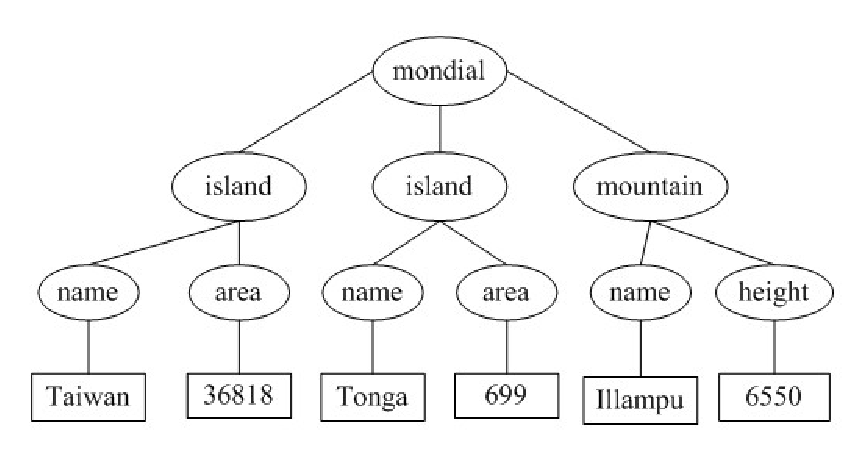
\includegraphics[width=0.4\textwidth]{XML}
\caption{树状结构}\label{fig:xml}
\vspace{\baselineskip}
\end{figure}


其插入图片的代码及其说明如下。
\vspace{1em}\noindent\hrule
\begin{verbatim}
\begin{figure}[htbp]
\centering
\includegraphics[width=0.4\textwidth]{文件名(.eps)}
\caption{标题}\label{标签名(通常为 fig:labelname)}
\vspace{\baselineskip} %表示图与正文空一行
\end{figure}
\end{verbatim}

\noindent\hrule

\begin{verbatim}
figure环境的可选参数[htbp]表示浮动图形所放置的位置,h (here)表示当前位置,t (top)表示页芯顶部,b (bottom)表示页芯底部,p (page)表示单独一页。在Word等软件中,图片通常插入到当前位置,如果当前页的剩余空间不够,图片将被移动到下一页,当前页就会出现很大的空白,其人工调整工作非常不便。由LaTeX提供的浮动图片功能,总是会按h->t->b->p的次序处理选项中的字母,自动调整图片的位置,大大减轻了工作量。
\centering命令将后续内容转换成每行皆居中的格式。
"\includegraphics"的可选参数用来设置图片插入文中的水平宽度,一般表示为正文宽度(\textwidth)的倍数。
\caption命令可选参数“标签名”为英文形式,一般不以图片或表格的数字顺序作为标签,而应包含一定的图片或表格信息,以便于文中引用(若图片、表格、公式、章节和参考文献等在文中出现的先后顺序发生了变化,其标注序号及其文中引用序号也会跟着发生变化,这一点是Word等软件所不能做到的)。另外,图题或表题并不会因为分页而与图片或表格体分置于两页,章节等各级标题也不会置于某页的最底部,LaTeX系统会自动调整它们在正文中的位置,这也是Word等软件所无法匹敌的。
\vspace将产生一定高度的竖直空白,必选参数为负值表示将后续文字位置向上提升,参数值可自行调整。em为长度单位,相当于大写字母M的宽度。\vspace{\baselineskip} 表示图与正文空一行。
引用方法:“见图~\ref{fig:figname}”、“如图~\ref{fig:figname}~所示”等。
\end{verbatim}

\noindent\hrule\vspace{1em}

若需要将~2~张及以上的图片并排插入到一行中,则需要采用\verb|minipage|环境,如图~\ref{fig:dd}~和图~\ref{fig:ds}~所示。
\begin{figure}[htbp]
\centering
\begin{minipage}{0.4\textwidth}
\centering
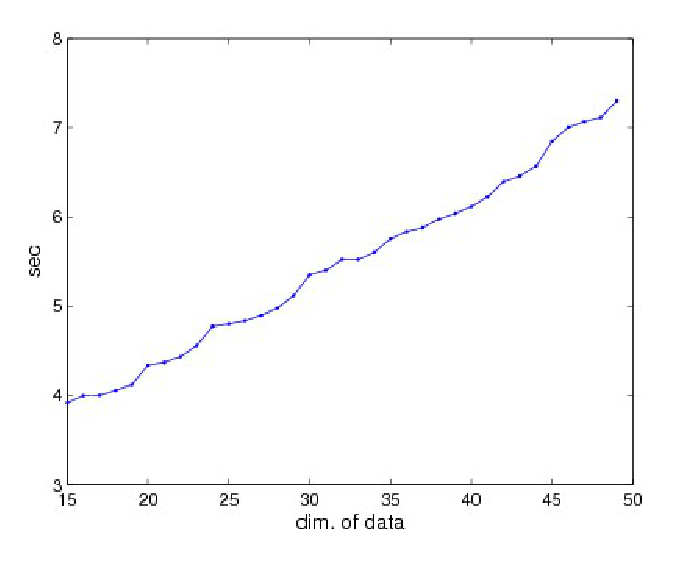
\includegraphics[width=\textwidth]{dataDimensions}
\caption{数据维数的变化}\label{fig:dd}
\end{minipage}
\begin{minipage}{0.4\textwidth}
\centering
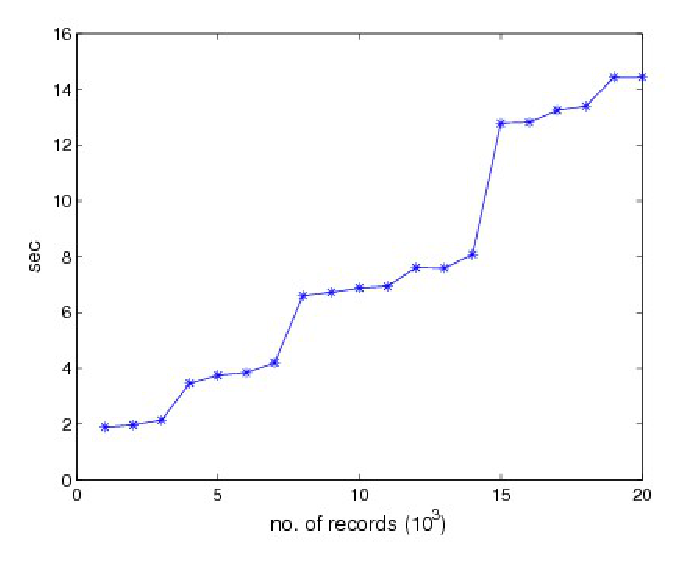
\includegraphics[width=\textwidth]{dataSize}
\caption{数据规模的变化}\label{fig:ds}
\end{minipage}
\vspace{\baselineskip}
\end{figure}

其代码如下所示。
\vspace{1em}\noindent\hrule
\begin{verbatim}
\begin{figure}[htbp]
\centering
\begin{minipage}{0.4\textwidth}
\centering
\includegraphics[width=\textwidth]{文件名}
\caption{标题}\label{fig:f1}
\end{minipage}
\begin{minipage}{0.4\textwidth}
\centering
\includegraphics[width=\textwidth]{文件名}
\caption{标题}\label{fig:f2}
\end{minipage}\vspace{\baselineskip}
\end{figure}
\end{verbatim}

\noindent\hrule

\begin{verbatim}
minipage环境的必选参数用来设置小页的宽度,若需要在一行中插入n个等宽图片,则每个小页的宽度应略小于(1/n)\textwidth。
\end{verbatim}

\noindent\hrule

\section{具有子图的图片插入方法}

图中若含有子图时,需要调用~subfigure~宏包, 如图~\ref{fig:subfig}~所示。
\begin{figure}[htbp]
  \centering
  \subfigure[Data Dimensions]{\label{fig:subfig:datadim}
                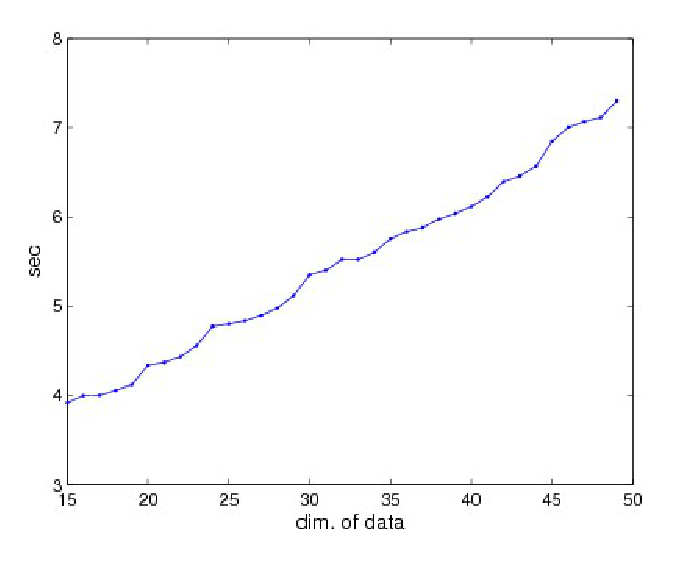
\includegraphics[width=0.4\textwidth]{dataDimensions}}
  \subfigure[Data Size]{\label{fig:subfig:datasize}
                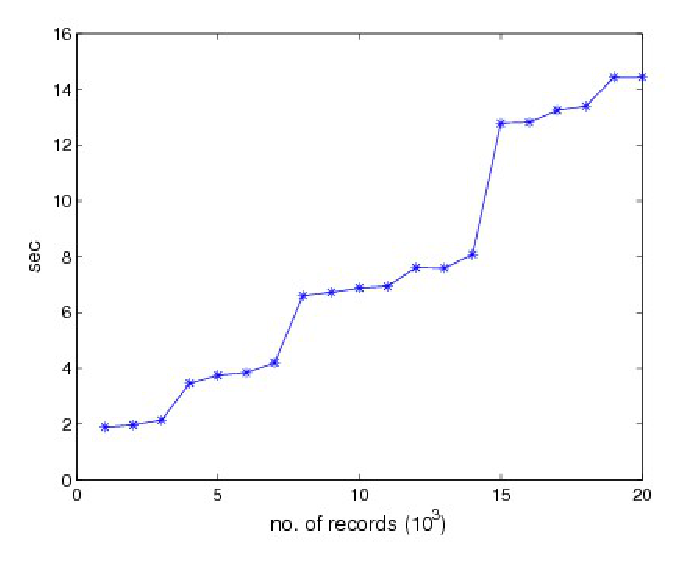
\includegraphics[width=0.4\textwidth]{dataSize}}
  \caption{Scalability of data}\label{fig:subfig}
\vspace{\baselineskip}
\end{figure}

其代码及其说明如下。
\vspace{1em}\noindent\hrule

\begin{verbatim}
\begin{figure}[htbp]
  \centering
  \subfigure[第1个子图标题]{
            \label{第1个子图标签(通常为 fig:subfig1:subsubfig1)}
            \includegraphics[width=0.4\textwidth]{文件名}}
  \subfigure[第2个子图标题]{
            \label{第2个子图标签(通常为 fig:subfig1:subsubfig2)}
            \includegraphics[width=0.4\textwidth]{文件名}}
  \caption{总标题}\label{总标签(通常为 fig:subfig1)}
\vspace{\baselineskip}
\end{figure}
\end{verbatim}

\noindent\hrule

\begin{verbatim}
子图的标签实际上可以随意设定,只要不重复就行。但为了更好的可读性,我们建议fig:subfig:subsubfig格式命名,这样我们从标签名就可以知道这是一个子图引用。
引用方法:总图的引用方法同本章第1节,子图的引用方法用\ref{fig:subfig:subsubfig}来代替。
\end{verbatim}

\noindent\hrule\vspace{1em}

子图的引用示例:如图~\ref{fig:subfig:datadim}~和图~\ref{fig:subfig:datasize}~所示。

若想获得插图方法的更多信息,参见网络上的~\href{ftp://ftp.tex.ac.uk/tex-archive/info/epslatex.pdf}{Using Imported Graphics in \LaTeX and pdf\LaTeX}~文档。 
%%% !Mode:: "TeX:UTF-8"

\chapter{表格的绘制方法}
\section{研究生毕业设计论文的绘表规范}

表应有自明性。表格不加左、右边线。表的编排建议采用国际通行的三线表。表内中文书写使用宋体五号字。

每个表格之上均应有表题(由表序和表名组成)。表序一般按章编排,如第~1~章第一个插表的序号为“表~1-1”等。表序与表名之间空两格,
表名使用中文五号字,居中。表名中不允许使用标点符号,表名后不加标点。
表头设计应简单明了,尽量不用斜线。表头中可采用化学,物理量等专业符号。

全表如用同一单位,则将单位符号移至表头右上角,加圆括号。
表中数据应准确无误,书写清楚。数字空缺的格内加横线“-”(占~2~个数字宽度)。表内文字或数字上、下或左、右相同时,
采用通栏处理方式,不允许用“〃”、“同上”之类的写法。

表内文字使用宋体五号字,垂直居中书写,起行空一格、转行顶格、句末不加标点。
如某个表需要转页接排,在随后的各页上应重复表的编号。编号后加“(续表)”,表题可省略。续表应重复表头。
表格绘制完成之后,与正文空一行。

\section{普通表格的绘制方法}

表格应具有三线表格式,因此需要调用~booktabs~宏包,其标准格式如表~\ref{tab:table1}~所示。
\begin{table}[htbp]
\caption{符合本科生毕业论文绘图规范的表格}\label{tab:table1}
\vspace{0.5em}\centering\wuhao
\begin{tabular}{ccccc}
\toprule[1.5pt]
$D$(in) & $P_u$(lbs) & $u_u$(in) & $\beta$ & $G_f$(psi.in)\\
\midrule[1pt]
 5 & 269.8 & 0.000674 & 1.79 & 0.04089\\
10 & 421.0 & 0.001035 & 3.59 & 0.04089\\
20 & 640.2 & 0.001565 & 7.18 & 0.04089\\
 5 & 269.8 & 0.000674 & 1.79 & 0.04089\\
10 & 421.0 & 0.001035 & 3.59 & 0.04089\\
20 & 640.2 & 0.001565 & 7.18 & 0.04089\\
 5 & 269.8 & 0.000674 & 1.79 & 0.04089\\
10 & 421.0 & 0.001035 & 3.59 & 0.04089\\
20 & 640.2 & 0.001565 & 7.18 & 0.04089\\
 5 & 269.8 & 0.000674 & 1.79 & 0.04089\\
10 & 421.0 & 0.001035 & 3.59 & 0.04089\\
20 & 640.2 & 0.001565 & 7.18 & 0.04089\\
\bottomrule[1.5pt]
\end{tabular}
\vspace{\baselineskip}
\end{table}

其绘制表格的代码及其说明如下。
\vspace{1em}\noindent\hrule

\begin{verbatim}
\begin{table}[htbp]
\caption{表标题}\label{标签名(通常为 tab:tablename)}
\vspace{0.5em}\centering\wuhao
\begin{tabular}{cc...c}
\toprule[1.5pt]
表头第1个格   & 表头第2个格   & ... & 表头第n个格  \\
\midrule[1pt]
表中数据(1,1) & 表中数据(1,2) & ... & 表中数据(1,n)\\
表中数据(2,1) & 表中数据(2,2) & ... & 表中数据(2,n)\\
表中数据(3,1) & 表中数据(3,2) & ... & 表中数据(3,n)\\
表中数据(4,1) & 表中数据(4,2) & ... & 表中数据(4,n)\\
...................................................\\
表中数据(m,1) & 表中数据(m,2) & ... & 表中数据(m,n)\\
\bottomrule[1.5pt]
\end{tabular}
\vspace{\baselineskip}
\end{table}
\end{verbatim}

\noindent\hrule

\begin{verbatim}
table环境是一个将表格嵌入文本的浮动环境。
\wuhao命令将表格的字号设置为五号字(10.5pt),在绘制表格结束退出时,不需要将字号再改回为\xiaosi,正文字号默认为小四号字(12pt)。
tabular环境的必选参数由每列对应一个格式字符所组成:c表示居中,l表示左对齐,r表示右对齐,其总个数应与表的列数相同。此外,@{文本}可以出现在任意两个上述的列格式之间,其中的文本将被插入每一行的同一位置。表格的各行以\\分隔,同一行的各列则以&分隔。
\toprule、\midrule和\bottomrule三个命令是由booktabs宏包提供的,其中\toprule和\bottomrule分别用来绘制表格的第一条(表格最顶部)和第三条(表格最底部)水平线,\midrule用来绘制第二条(表头之下)水平线,且第一条和第三条水平线的线宽为1.5pt,第二条水平线的线宽为1pt。
引用方法:“如表~\ref{tab:tablename}~所示”。
\end{verbatim}

\noindent\hrule

\section{长表格的绘制方法}

长表格是当表格在当前页排不下而需要转页接排的情况下所采用的一种表格环境。若长表格仍按照普通表格的绘制方法来获得,
其所使用的\verb|table|浮动环境无法实现表格的换页接排功能,表格下方过长部分会排在表格第1页的页脚以下。为了能够实现长表格的转页接排功能,
需要调用~longtable~宏包,由于长表格是跨页的文本内容,因此只需要单独的\verb|longtable|环境,所绘制的长表格的格式如表~\ref{tab:table2}~所示。

此长表格~\ref{tab:table2}~第~2~页的标题“编号(续表)”和表头是通过代码自动添加上去的,无需人工添加,若表格在页面中的竖直位置发生了变化,长表格在第~2~页
及之后各页的标题和表头位置能够始终处于各页的最顶部,也无需人工调整,\LaTeX~系统的这一优点是~Word~等软件所无法企及的。

下段内容是为了让下面的长表格分居两页,看到表标题“编号(续表)”的效果。摘录于《你若安好,便是晴天 -- 林徽因传》片段:

她叫林徽因,出生于杭州,是许多人梦中期待的白莲。她在雨雾之都伦敦,发生过一场空前绝后的康桥之恋。她爱过三个男子,爱得清醒,也爱得平静。徐志摩为她徜徉在康桥,深情地等待一场旧梦可以归来。梁思成与她携手走过千山万水,为完成使命而相约白头。金岳霖为她终身不娶,痴心不改地守候一世。可她懂得人生飘忽不定,要学会随遇而安。
真正的平静,不是避开车马喧嚣,而是在心中修篱种菊。尽管如流往事,每一天都涛声依旧,只要我们消除执念,便可寂静安然。愿每个人在纷呈世相中不会迷失荒径,可以端坐磐石上,醉倒落花前。
如果可以,请让我预支一段如莲的时光,哪怕将来某一天加倍偿还。这个雨季会在何时停歇,无从知晓。但我知道,你若安好,便是晴天。					
\wuhao\begin{longtable}{ccc}
\caption{天津大学各学院名称一览}\label{tab:table2}
 \vspace{0.5em}\\
\toprule[1.5pt] 学院名称 & 网址 & 联系电话  \\ \midrule[1pt]
\endfirsthead
\multicolumn{3}{c}{表~\thetable(续表)}\vspace{0.5em}\\
\toprule[1.5pt] 学院名称 & 网址 & 联系电话  \\ \midrule[1pt]
\endhead
\bottomrule[1.5pt]
\endfoot
机械工程学院& \url{http://tdjxxy.tju.edu.cn/}& 87401979\\
精密仪器与光电子工程学院&  \url{http://www2.tju.edu.cn/colleges/precision/cn/}& 27404775\\
电子信息工程学院& \url{http://www.tju.edu.cn/seie}& 27406956\\
电气与自动化工程学院& \url{http://www2.tju.edu.cn/colleges/automate/}& 27405477\\
建筑工程学院& \url{http://www2.tju.edu.cn/colleges/civil/}& 27404072\\
化工学院& \url{http://chemeng.tju.edu.cn/}& 27403389\\
材料科学与工程学院& \url{http://mse.tju.edu.cn}& 27406693 \\
建筑学院& \url{http://hgw022072.chinaw3.com/}& 27402724-2111\\
求是学部\\
管理与经济学部&	\url{ http://sm.tju.edu.cn}& 27403423\\
理学院& \url{ http://www.tju.edu.cn/science/}& 27404118\\
文法学院& \url{ http://www2.tju.edu.cn/colleges/sociology/new/}& 27403691\\
软件学院& \url{http://scs.tju.edu.cn}& 87401540\\
计算机科学与技术学院& \url{http://cs.tju.edu.cn/}& 27406538\\
马克思主义学院& \url{http://www2.tju.edu.cn/colleges/marxism/}& 27405348\\
环境科学与工程学院& \url{http://www.tju.edu.cn/see}& 87402072\\
药物科学与技术学院& \url{http://www2.tju.edu.cn/colleges/pharmtier/}& 87401830\\
教育学院& \url{http://soe.tju.edu.cn/}& 27401028\\
职业技术教育学院& \url{http://202.113.0.248:8888}\\
继续教育学院& \url{http://aectu.tju.edu.cn/}& 27406298\\
仁爱学院& \url{http://www.tjrac.edu.cn/}& 68579990\\
农业与生物工程学院& \url{http://202.113.13.169/site/nongxueyuan/}& 87402171\\
国际教育学院 & \url{http://www.ietju.com/}& 27406147\\
网络教育学院 & \url{http://www.etju.com/}& 27426952 \\

\end{longtable}\xiaosi
\vspace{\baselineskip}

绘制长表格的代码及其说明如下。
\vspace{1em}\noindent\hrule

\begin{verbatim}
\wuhao\begin{longtable}{cc...c}
\caption{表标题}\label{标签名(通常为 tab:tablename)}\\
\toprule[1.5pt] 表头第1个格 & 表头第2个格 & ... & 表头第n个格\\ \midrule[1pt]
\endfirsthead
\multicolumn{n}{c}{表~\thetable(续表)}\vspace{0.5em}\\
\toprule[1.5pt] 表头第1个格 & 表头第2个格 & ... & 表头第n个格\\ \midrule[1pt]
\endhead
\bottomrule[1.5pt]
\endfoot
表中数据(1,1) & 表中数据(1,2) & ... & 表中数据(1,n)\\
表中数据(2,1) & 表中数据(2,2) & ... & 表中数据(2,n)\\
...................................................\\
表中数据(m,1) & 表中数据(m,2) & ... & 表中数据(m,n)\\
\end{longtable}\xiaosi
\end{verbatim}

\noindent\hrule
\begin{verbatim}
在绘制长表格的前面留出一个空白行,并在第2行的一开始全局定义长表格的字号为五号字,这样能够保证长表格之前段落的行距保持不变。
在绘制长表格结束后,需要\xiaosi命令重新将字号改为小四号字。
\endhead之前的文字描述的是第2页及其之后各页的标题或表头;
\endfirsthead之前的文字描述的是第1页的标题和表头,若无此命令,则第1页的表头和标题由\endhead命令确定;
同理,\endfoot之前的文字描述的是除最后一页之外每页的表格底部内容;
\endlastfoot之前的文字描述的是最后一页的表格底部内容,若无此命令,
则最后一页的表格底部内容由\endfoot命令确定;由于规范中长表格每页底部内容均相同(水平粗线),因此模板中没有用到\endlastfoot命令。
\end{verbatim}

\noindent\hrule
\section{列宽可调表格的绘制方法}
论文中能用到列宽可调表格的情况共有两种:一种是当插入的表格某一单元格内容过长以至于一行放不下的情况,
另一种是当对公式中首次出现的物理量符号进行注释的情况。这两种情况都需要调用~tabularx~宏包。下面将分别对这两种情况下可调表格的绘制方法进行阐述。
\subsection{表格内某单元格内容过长的情况}

首先给出这种情况下的一个例子如表~\ref{tab:table3}~所示。
\begin{table}[htbp]
\caption{最小的三个正整数的英文表示法}\label{tab:table3}
\vspace{0.5em}\wuhao
\begin{tabularx}{\textwidth}{llX}
\toprule[1.5pt]
Value & Name & Alternate names, and names for sets of the given size\\\midrule[1pt]
1 & One & ace, single, singleton, unary, unit, unity\\
2 & Two & binary, brace, couple, couplet, distich, deuce, double, doubleton, duad, duality, duet, duo, dyad, pair, snake eyes, span, twain, twosome, yoke\\
3 & Three & deuce-ace, leash, set, tercet, ternary, ternion, terzetto, threesome, tierce, trey, triad, trine, trinity, trio, triplet, troika, hat-trick\\\bottomrule[1.5pt]
\end{tabularx}
\vspace{\baselineskip}
\end{table}
绘制这种表格的代码及其说明如下。
\vspace{1em}\noindent\hrule
\begin{verbatim}
\begin{table}[htbp]
\caption{表标题}\label{标签名(通常为 tab:tablename)}
\vspace{0.5em}\wuhao
\begin{tabularx}{\textwidth}{l...X...l}
\toprule[1.5pt]
表头第1个格   & ... & 表头第X个格   & ... & 表头第n个格  \\
\midrule[1pt]
表中数据(1,1) & ... & 表中数据(1,X) & ... & 表中数据(1,n)\\
表中数据(2,1) & ... & 表中数据(2,X) & ... & 表中数据(2,n)\\
.........................................................\\
表中数据(m,1) & ... & 表中数据(m,X) & ... & 表中数据(m,n)\\
\bottomrule[1.5pt]
\end{tabularx}
\vspace{\baselineskip}
\end{table}
\end{verbatim}

\noindent\hrule
\begin{verbatim}
tabularx环境共有两个必选参数:第1个参数用来确定表格的总宽度,这里取为排版表格能达到的最大宽度——正文宽度\textwidth;第2个参数用来确定每列格式,其中标为X的项表示该列的宽度可调,其宽度值由表格总宽度确定。
标为X的列一般选为单元格内容过长而无法置于一行的列,这样使得该列内容能够根据表格总宽度自动分行。若列格式中存在不止一个X项,则这些标为X的列的列宽相同,因此,一般不将内容较短的列设为X。
标为X的列均为左对齐,因此其余列一般选为l(左对齐),这样可使得表格美观,但也可以选为c或r。
\end{verbatim}

\noindent\hrule
\subsection{对物理量符号进行注释的情况}
为使得对公式中物理量符号注释的转行与破折号“———”后第一个字对齐,此处最好采用表格环境。此表格无任何线条,左对齐,
且在破折号处对齐,一共有“式中”二字、物理量符号和注释三列,表格的总宽度可选为文本宽度,因此应该采用\verb|tabularx|环境。
由\verb|tabularx|环境生成的对公式中物理量符号进行注释的公式如式(\ref{eq:1})所示。
%\vspace*{10pt}

\begin{equation}\label{eq:1}
\ddot{\boldsymbol{\rho}}-\frac{\mu}{R_{t}^{3}}\left(3\mathbf{R_{t}}\frac{\mathbf{R_{t}\rho}}{R_{t}^{2}}-\boldsymbol{\rho}\right)=\mathbf{a}
\end{equation}

\begin{tabularx}{\textwidth}{@{}l@{\quad}r@{———}X@{}}
式中& $\bm{\rho}$ &追踪飞行器与目标飞行器之间的相对位置矢量;\\
&  $\bm{\ddot{\rho}}$&追踪飞行器与目标飞行器之间的相对加速度;\\
&  $\mathbf{a}$   &推力所产生的加速度;\\
&  $\mathbf{R_t}$ & 目标飞行器在惯性坐标系中的位置矢量;\\
&  $\omega_{t}$ & 目标飞行器的轨道角速度;\\
&  $\mathbf{g}$ & 重力加速度,$=\frac{\mu}{R_{t}^{3}}\left(
3\mathbf{R_{t}}\frac{\mathbf{R_{t}\rho}}{R_{t}^{2}}-\bm{\rho}\right)=\omega_{t}^{2}\frac{R_{t}}{p}\left(
3\mathbf{R_{t}}\frac{\mathbf{R_{t}\rho}}{R_{t}^{2}}-\bm{\rho}\right)$,这里~$p$~是目标飞行器的轨道半通径。
\end{tabularx}
\vspace{\wordsep}

其中生成注释部分的代码及其说明如下。

\vspace{1em}\noindent\hrule

\begin{verbatim}
\begin{tabularx}{\textwidth}{@{}l@{\quad}r@{— — —}X@{}}
式中 & symbol-1 & symbol-1的注释内容;\\
     & symbol-2 & symbol-2的注释内容;\\
     .............................;\\
     & symbol-m & symbol-m的注释内容。
\end{tabularx}\vspace{\wordsep}
\end{verbatim}

\noindent\hrule

\begin{verbatim}
tabularx环境的第1个参数选为正文宽度,第2个参数里面各个符号的意义为:
    第1个@{}表示在“式中”二字左侧不插入任何文本,“式中”二字能够在正文中左对齐,若无此项,则“式中”二字左侧会留出一定的空白;
    @{\quad}表示在“式中”和物理量符号间插入一个空铅宽度的空白;
    @{— — —}实现插入破折号的功能,它由三个1/2的中文破折号构成;
    第2个@{}表示在注释内容靠近正文右边界的地方能够实现右对齐。
\end{verbatim}

\noindent\hrule\vspace{1em}

由此方法生成的注释内容应紧邻待注释公式并置于其下方,因此不能将代码放入\verb|table|浮动环境中。但此方法不能实现自动转页接排,
可能会在当前页剩余空间不够时,全部移动到下一页而导致当前页出现很大空白。因此在需要转页处理时,还请您手动将需要转页的代码放入一个
新的\verb|tabularx|环境中,将原来的一个\verb|tabularx|环境拆分为两个\verb|tabularx|环境。

若想获得绘制表格的更多信息,参见网络上的~\href{http://www.tug.org/pracjourn/2007-1/mori/}{Tables in \LaTeXe: Packages and Methods}~文档。


%%\include{body/equations}
%%% !Mode:: "TeX:UTF-8"

\chapter{罗列和定理环境使用方法}

\section{单层罗列环境}
天津大学学位论文一般可采用两种罗列环境:一种是并列条目有同样标签的~\verb|itemize|~罗列环境,另一种是具有自动排序编号符号的~\verb|enumerate|~罗列环境。这两种罗列环境的样式参数可参考图~\ref{fig:list}。
\begin{figure}[htbp]
\centering
\includegraphics[width = 0.6\textwidth]{list}
\caption{罗列环境参数示意图}\label{fig:list}\vspace{-1em}
\end{figure}

通过调用~enumitem~宏包可以很方便地控制罗列环境的布局,其~format.tex~文件中的~\verb|\setitemize|~和~\verb|\setenumerate|~命令分别用来设置~\verb|itemize|~和~\verb|enumerate|~环境的样式参数。采用~\verb|itemize|~单层罗列环境的排版形式如下:

\begin{itemize}
\item 第一个条目文本内容
\item 第二个条目文本内容
\item 第三个条目文本内容
\end{itemize}

其代码如下

\begin{verbatim}
\begin{itemize}
  \item 第一个条目文本内容
  \item 第二个条目文本内容
  ...
  \item 第三个条目文本内容
\end{itemize}
\end{verbatim}

采用~\verb|enumerate|~单层罗列环境的排版形式如下:

\begin{enumerate}
\item 第一个条目文本内容
\item 第二个条目文本内容
\item 第三个条目文本内容
\end{enumerate}

其代码如下

\begin{verbatim}
\begin{enumerate}
  \item 第一个条目文本内容
  \item 第二个条目文本内容
  ...
  \item 第三个条目文本内容
\end{enumerate}
\end{verbatim}



\section{定理环境}

\begin{definition}[谱半径]\label{def:def1}
  称~$n$~阶方阵~$\mathbf{A}$~的全体特征值~$\lambda_1,\cdots,\lambda_n$~组成的集合为~$\mathbf{A}$~的谱,称
  $$\rho(\mathbf{A})=\max{\{|\lambda_1|,\cdots,|\lambda_n|\}}$$
\end{definition}
\begin{theorem}[相似充要条件]\label{lemma:l1}
  方阵$A$和$B$相似的充要条件是:~$A$~和~$B$~有全同的不变因子。
\end{theorem}
\begin{corollary}[推论1]\label{cor:cor1}
在赋范空间~$(X,\|\cdot\|)$~上定义~$d(x,y)=\|x-y\|$, 对任意~$x,y\in X$,~则~$(X,d)$~是距离空间。
\end{corollary}
\begin{proof}
  只需证明~$d(x,y)$~是距离。
\end{proof}
\newpage

定义代码如下:
\begin{verbatim}
 \begin{definition}[谱半径]\label{def:def1}
  称~$n$~阶方阵~$\mathbf{A}$~的全体特征值
  $\lambda_1,\cdots,\lambda_n$组成的集合为~$\mathbf{A}$~的谱,称
  $$\rho(\mathbf{A})=\max{\{|\lambda_1|,\cdots,|\lambda_n|\}}$$
\end{definition}
\end{verbatim}
\noindent\hrule

\vspace{0.1em}\noindent\hrule
\vspace{1em}
定理代码如下:
\begin{verbatim}
\begin{theorem}[相似充要条件]\label{lemma:l1}
  方阵$A$和$B$相似的充要条件是:$A$和$B$有全同的不变因子。
\end{theorem}
\end{verbatim}
\noindent\hrule\vspace{0.1em}

\noindent\hrule
\vspace{1em}
推论和证明代码如下:
\begin{verbatim}
\begin{corollary}[推论1]\label{cor:cor1}
在赋范空间~$(X,\|\cdot\|)$~上定义$d(x,y)=\|x-y\|$,
对任意$x,y\in X$,则$(X,d)$是距离空间。
\end{corollary}
\begin{proof}
  只需证明$d(x,y)$是距离。
\end{proof}
\end{verbatim}
\noindent\hrule\vspace{1em}

定理定义[]中是可选参数,用来说明定理的名称。其他环境格式书写与上面定理、定义、推论格式相同,可自己调用其他环境。
若需要书写定理定义等内容,而且带有顺序编号,需要采用如下环境。除了~\verb|proof|~环境之外,其余~9~个环境都可以有一个可选参数作为附加标题。

\begin{center}
\vspace{0.5em}\noindent\wuhao\begin{tabularx}{0.7\textwidth}{lX|lX}
定理 & \verb|theorem|~环境 & 定义 & \verb|definition|~环境 \\
例 & \verb|example|~环境 & 算法 & \verb|algorithm|~环境 \\
公理 & \verb|axiom|~环境 & 命题 & \verb|proposition|~环境 \\
引理 & \verb|lemma|~环境 & 推论 & \verb|corollary|~环境 \\
注解 & \verb|remark|~环境 & 证明 & \verb|proof|~环境 \\
\end{tabularx}
\end{center} 
%%\include{body/conclusion}
\end{verbatim}
那么,编译的时候就只编译未加~\%~的一章,在这个例子中,即本章~intros。

理论上,并不一定要把每章放在不同的文件中。但是这种自顶向下,分章节写作、编译的方法有利于提高效率,大大减少~Debug~过程中的编译时间,同时减小风险。

\section{参考文献生成方法}

\LaTeX~具有插入参考文献的能力。Google Scholar~网站上存在兼容~BibTeX~的参考文献信息,通过以下几个步骤,可以轻松完成参考文献的生成。
\begin{itemize}
  \item 在\href{http://scholar.google.com/}{谷歌学术搜索}中,
        点击\href{http://scholar.google.com/scholar_preferences?hl=en&as_sdt=0,5}{学术搜索设置}。
  \item 页面打开之后,在\textbf{文献管理软件}选项中选择\textbf{显示导入~BibTeX~的链接},单击保存设置,退出。
  \item 在谷歌学术搜索中检索到文献后,在文献条目区域单击导入~BibTeX~选项,页面中出现文献的引用信息。
  \item 将文献引用信息的内容复制之后,添加到~references~文件夹下的~reference.bib~中。
\end{itemize}

\section{编译注意事项}
\begin{enumerate}
  \item 由于模板使用~UTF-8~编码,所以源文件应该保存成~UTF-8~格式,否则可能出现中文字符无法识别的错误。
  本模板中每一个~.tex~文件的文件的开头已经加上一行:\\
    \verb|% !Mode:: "TeX:UTF-8"|\\
     这样可以确保~.tex~文件默认使用~UTF-8~的格式打开。读者如果删去此行,很有可能会导致中文字符显示乱码。
     在~WinEdt~编辑器中可以使用以下两种方式保存成~UTF-8~格式:
      \begin{enumerate}
        \item 先建立~.tex~文件,另存为~.tex~文件时,选择用~UTF-8~格式保存。
        \item
            在~WinEdt~编辑器中,选择\\
            \mbox{~Document$\to$Document Settings$\to$Document Mode $\to$TeX:UTF-8} 同时在~WinEdt~最下面的状态栏中,可以看到该文档是~TeX~格式还是~TeX:UTF-8~格式。
            当文档为~TeX:UTF-8~格式时,状态栏一般显示:
            \makebox[\textwidth][l]{Wrap | Indent | INS | LINE |Spell | TeX:UTF-8 | -src~等。}
      \end{enumerate}
  \item 如果在pdf书签中,中文显示乱码的话,则注意以下说明:
    \begin{verbatim}
        \usepackage{CJKutf8}
        % 1. 如果使用CJKutf8
        %    Hyperref中应使用unicode参数
        % 2. 如果使用CJK
        %    Hyperref则使用CJKbookmarks参数
        %    可惜得到的PDF书签是乱码,建议弃用
        % 3. Unicode选项和CJKbookmarks不能同时使用
        \usepackage[
        %CJKbookmarks=true,
        unicode=true
        ]{hyperref}
     \end{verbatim}
 \item 建议采用以下两种编译方式:
  \begin{enumerate}
     \item latex + bibtex + latex + latex + dvi2pdf. 在这种编译情况下,对应的~tjumain.tex~文件的第一行是\verb|\def\usewhat{dvipdfmx}|~(缺省设置)。 此时,所有图片文件应该保存为~.eps~格式,如~figures~文件夹里~.eps~图片。
          如果您选择在命令行中操作,可以在编译的时候依次输入~latex tjumain, bibtex tjumain, latex tjumain, latex tjumain~和~dvipdfmx tjumain, 编译完成之后,需要手动打开~pdf~文件。
     \item pdflatex + pdflatex. 在这种编译情况下,对应的~tjumain.tex~文件的第一行应该改为\verb|\def\usewhat{pdflatex}|~。 此时, 编译不支持~.eps~图片格式,此时需要在命令行下使用~epstopdf~指令将~figures~文件夹下 的~.eps~文件转化成~.pdf~文件格式,命令行中操作格式为~epstopdf a.eps~。
          在命令行编译的时候,依次输入~pdflatex tjumain~和~pdflatex tjumain, 编译完成之后,需要手动打开~pdf~文件。
  \end{enumerate}
\end{enumerate}

\section{系统要求}
    CTEX 2.8, MiKTeX 2.8, TeX Live 2009~或以上版本。使用推荐的~WinEdt 6.0~编辑器,可以完成文件的编辑和编译工作。

\section{\TeX~简介}

以下内容是~milksea@bbs.ctex.org~撰写的关于~\TeX~的简单介绍,略有改动。
注意这不是一个入门教程,不讲~\TeX~系统的配置安装,也不讲具体的~\LaTeX~代码。
这里仅仅试图以一些只言片语来解释:
进入这个门槛之前新手应该知道的注意事项,以及遇到问题以后该去如何解决问题。

\subsection{什么是 \TeX/\LaTeX,我是否应该选择它~?}

\TeX~是最早由高德纳(Donald Knuth)教授创建的一门标记式宏语言,
用来排版科技文章,尤其擅长处理复杂的数学公式。\TeX~同时也是处理这一语言的排版软件。
\LaTeX~是 Leslie Lamport 在~\TeX~基础上按内容/格式分离和模块化等思想建立的一集~\TeX~上的格式。

\TeX~本身的领域是专业排版领域
但现在~TeX/LaTeX~也被广泛用于生成电子文档甚至幻灯片等,~\TeX~语言的数学部分
偶尔也在其他一些地方使用。但注意~\TeX~并不适用于文书处理(Microsoft Office 的领域,以前和现在都不是)。

选择使用~\TeX/\LaTeX~的理由包括:
\begin{itemize}
\item 免费软件;
\item 专业的排版效果;
\item 是事实上的专业数学排版标准;
\item 广泛的西文期刊接收甚或只接收 LaTeX 格式的投稿;
\item[] ……
\end{itemize}
不选择使用~\TeX/\LaTeX~的理由包括:
\begin{itemize}
\item 需要相当精力学习;
\item 图文混合排版能力不够强;
\item 仅在数学、物理、计算机等领域流行;
\item 中文期刊的支持较差;
\item[] ……
\end{itemize}

请尽量清醒看待网上经常见到的关于~\TeX~与其他软件的优劣比较和口水战。在选择使用或离开之前,请先考虑
\TeX~的应用领域,想想它是否适合你的需要。


\subsection{我该用什么编辑器~?}

编辑器功能有简有繁,特色不一,从简单的纯文本编辑器到繁复的 Emacs,因人而易。基本功能有语法高亮、方便编译预览就很好了,扩充功能和定制有无限的可能。初学者可以使用功能简单、使用方便的专用编辑器,如 ~TeXWorks、Kile、WinEdt~等,或者类似所见即所得功能的~LyX;熟悉的人可以使用定制性更强的~Notepad++、SciTE、Vim、Emacs ~等。这方面的介绍很多,一开始不妨多试几种,找到最适合自己的才是最好的。

另外提醒一句,编辑器只是工作的助手,不必把它看得太重。

\subsection{我应该看什么~\LaTeX~读物~?}

这不是一个容易回答的问题,因为有许多选择,也同样有许多不合适的选择。
这里只是选出一个比较好的答案。更多更详细的介绍可以在版面和网上寻找(注意时效)。

近两年~\TeX~的中文处理发展很快,目前没有哪本书在中文处理方面给出一个最新进展的合适综述,
因而下面的介绍也不主要考虑中文处理。

\begin{enumerate}

\item 我能阅读英文。
\begin{enumerate}
\item 迅速入门:ltxprimer.pdf (LaTeX Tutorials: A Primer, India TUG)
\item 系统学习:A Guide to LaTeX, 4th Edition, Addison-Wesley
               有机械工业出版社的影印版(《\LaTeX{}~实用教程》)
\item 深入学习:要读许多书和文档,TeXbook 是必读的
\item 细节学习:去读你使用的每一个宏包的说明文档
\item 专题学习:阅读讲数学公式、图形、表格、字体等的专题文档
\end{enumerate}

\item 我更愿意阅读中文。
\begin{enumerate}
\item 迅速入门:lnotes.pdf (LaTeX Notes, 1.20, Alpha Huang)
\item 系统学习:《\LaTeXe{}~科技排版指南》,邓建松(电子版)
      如果不好找,可以阅读《\LaTeXe~入门与提高》第二版,陈志杰等,或者 《\LaTeXe~完全学习手册》,胡伟
\item 深入学习:~TeXbook0.pdf~(特可爱原本,TeXbook 的中译,xianxian)
\item 具体问题释疑:~CTeX-FAQ.pdf~,\\
        吴凌云,~\url{http://www.ctex.org/CTeXFAQ}~
\end{enumerate}
\end{enumerate}

遇见问题和解决问题的过程可以快速提高自己的技能,建议此时:
\begin{itemize}
  \item 利用~Google~搜索。
  \item 清楚,扼要地提出你的问题。
\end{itemize}

\subsection{什么知识会过时~?什么不会~?}

\TeX~是排版语言,也是广泛使用的软件,并且不断在发展中;
因此,总有一些东西会很快过时。作为学习~\TeX~的人,
免不了要看各种各样的书籍、电子文档和网络论坛上的只言片语,
因此了解什么知识会迅速过时,什么知识不会是十分重要的。

最稳定的是关于~Primitive \TeX~和~Plain \TeX~的知识,也就是 Knuth
在他的《The TeXbook》中介绍的内容。因为~\TeX~
系统开发的初衷就是稳定性,要求今天的文档到很久以后仍可以得到完全相同的结果,
因此 Knuth 限定了他的~\TeX~语言和相关实现的命令、语法。这些内容许多年来就没有多少变化,
在未来的一些年里也不会有什么变化。
Primitive \TeX~和 Plain \TeX~的知识主要包括 \TeX~排版的基本算法和原理,
盒子的原理,底层的 \TeX~命令等。其中技巧性的东西大多在宏包设计中,
初学者一般不会接触到很多;而基本原理则是常常被提到的,
譬如,~\TeX~把一切排版内容作为盒子(box)处理。

相对稳定的是关于基本~\LaTeXe~
的知识,也包括围绕~\LaTeXe~的一些核心宏包的知识。~\LaTeXe~
是自~1993~年以来的一个稳定的~\LaTeX~版本,直到最近的一次修订
(2005 年)都没有大的变动。
\LaTeX~的下一个计划中的版本~\LaTeX 3~遥遥无期,在可预见的将来,~\LaTeXe~不会过时。
\LaTeXe~的知识是目前大部分~\LaTeX~书籍的主体内容。关于~\LaTeX~的标准文档类
~(article、report、book、letter、slide~等),关于基本数学公式的输入,
文档的章节层次,表格和矩阵,图表浮动体,LR 盒子与段落盒子……
这些~\LaTeX~的核心内容都是最常用的,相对稳定的。
与~\LaTeXe~相匹配的核心宏包,
如~graphics(x)、ifthen、fontenc、doc~等,也同样是相对稳定的。
还有一些被非常广泛应用的宏包,如~amsmath~系列,也可以看作是相对稳定的。

简单地说,关于基本~\TeX/\LaTeX~的语言,都是比较稳定的。与之对应,实现或者支持~\TeX/\LaTeX~语言的软件,
包括在~\TeX/\LaTeX~基础上建立的新的宏,都不大稳定。

容易过时的是关于第三方~\LaTeX~宏包的知识、第三方~\TeX~工具的知识,以及新兴~\TeX~相关软件的知识等。
~\TeX~和~\LaTeX~语言是追求稳定的;但无论是宏包还是工具,作为不断更新软件,它们是不稳定的。
容易过时的技术很多,而且现在广泛地出现在几乎所有~\LaTeX~文档之中,因此需要特别引起注意:
宏包的过时的原因可能是宏包本身的升级换代带来了新功能或不兼容,
也可能是同一功能的更新更好的宏包代替了旧的宏包。前者的典型例子比如绘图宏包~PGF/TikZ~,
现在的~2.00~版功能十分强大,和旧的~1.1x~版相差很大,和更旧的~0.x~版本则几乎完全不同;后
者的典型例子比如~caption~宏包先是被更新的~caption2~宏包代替,后来~caption~宏包更新又使得
caption2 宏包完全过时。——安装更新的发行版可以避免使用过旧的宏包;
认真阅读宏包自带的文档而不是搜索得到的陈旧片断可以避免采用过时的代码。

工具过时的主要原因也是升级换代和被其他工具替换。前者的典型例子是编辑器
WinEdt~在~5.5~以后的版本支持~UTF-8~编码,而旧版本不支持;
后者的典型例子是中文字体安装工具从~GBKFonts~到~xGBKFonts~到~FontsGen~不断被取代。
图形插入是一个在~\TeX~实现、宏包与外围工具方面都更新很快的东西。
在过去,最常用的输出格式是~PS(PostScript)~格式,因此插入的图像以~EPS~为主流。
使用~Dvips~为主要输出工具,外围工具有~GhostScript、bmeps~等等,相关宏包有~graphics~等,
相关文档如《\LaTeXe{}~ 插图指南》。

但凡提及“~\LaTeX~只支持~EPS~图形”的,就是这个过时的时代的产物。事实上~\TeX/\LaTeX~
并不限定任何图形格式,只不过是当时的输出格式(PS)和工具(Dvips)对~EPS~情有独钟而已。
后来 PDF 格式成为主流。~pdf\TeX、DVIPDFM、DVIPDFMx、XeTeX~工具则主要支持~PDF、PNG、JPG~格式的图形,
涉及一系列工具如~ImageMagick、ebb~等。

值得特别提出注意的就是,中文处理也一起是更新迅速、容易过时的部分。
而且因为中文处理一直没有一个“官方”的“标准”做法,软件、工具、
文档以及网上纷繁的笔记也就显得相当混乱。从八十年代开始的~CCT~系统、
天元系统,到后来的~CJK~方式,到近来的~XeTeX~和~LuaTeX~ 方式,
中文处理的原理、软件、宏包、配置方式等都在不断变化中。

\section{后期工作}
下表记录了~TJUThesis~计划中未来应该逐步实现的功能和特性:
\begin{enumerate}
  \item 编写更为详细的~TJUThesis~的使用手册和~FAQ~用户指南
  \item 加入对课程结课论文的支持
  \item 加入对天津大学学生经常参加的各种限时完成重大赛事的论文模板的支持,如全国研究生数学建模竞赛,以节省排版时间
  \item 加入对~pdf~书签中章节中文编号的支持,如: 第一章 XXX
  \item 加入对附录~A~等格式的支持
  \item Linux~平台迁移和测试
\end{enumerate}

\section{免责声明}

本模板依据《天津大学关于博士、硕士学位论文统一格式的规定》和《天津大学硕士论文模版》编写,适用于所有硕士生的学位论文编写。然而,作者不保证本模板完全符合学校要求,也不对由此带来的风险和损失承担任何责任。

%%% !Mode:: "TeX:UTF-8"

\chapter{图片的插入方法}

\section{博士学位论文的插图规范}

图应有自明性。插图应与文字紧密配合,文图相符,内容正确。选图要力求精练,插图、照片应完整清晰。图中文字和数字等字号用宋体五号字。

机械工程图:采用第一角投影法,严格按照~GB4457---GB131-83《机械制图》标准规定。

数据流程图、程序流程图、系统流程图等按~GB1526-89~标准规定。

电气图:图形符号、文字符号等应符合有关标准的规定。

流程图:必须采用结构化程序并正确运用流程框图。

对无规定符号的图形应采用该行业的常用画法。

坐标图的坐标线均用细实线,粗细不得超过图中曲线,有数字标注的坐标图,必须注明坐标单位。

照片图要求主题和主要显示部分的轮廓鲜明,便于制版。如用放大或缩小的复制品,必须清晰,反差适中。照片上应有表示目的物尺寸的标度。

引用文献图表必须标注出处。


\subsection{图题及图中说明}
每个图均应有图题(由图序和图名组成),图名在图序之后空两格排写。图序按章编排,如第~1~章第一个插图的图号为“图~1-1”等。
图题置于图下,要求中文用宋体五号字,位置居中。有图注或其它说明时应置于图题之上。引用图应注明出处,在图题右上角加引用文献号。
图中若有分图时,分图题置于分图之下或图题之下,分图号用~a)、b)等表示。

图中各部分说明应采用中文(引用的外文图除外)或数字项号,各项文字说明置于图题之上(有分图题者,置于分图题之上)。

\subsection{插图编排}
插图之前,文中必须有关于本插图的提示,如“见图~1-1”、“如图~1-1~所示”等。插图与其图题为一个整体,不得拆开排写于两页。
插图处的该页空白不够排写该图整体时,则可将其后文字部分提前排写,将图移到次页。

\section{\LaTeX~中推荐使用的图片格式}
在~\LaTeX~中应用最多的图片格式是~EPS(Encapsulated PostScript)格式,它是一种专用的打印机描述语言,常用于印刷或打印输出。
EPS~格式图片可通过多种方式生成,这里介绍一款功能强大的免费图片处理软件———\href{http://www.imagemagick.org/}{ImageMagick},
此软件可将其它格式图片转换为~EPS~格式图片,同时还可以锐化图片,使图片的局部清晰一些。

此软件对图片的格式转换操作都是在命令提示符(cmd.exe)中实现的,可以通过“开始$\to$运行$\to$输入~cmd$\to$回车”或
“开始$\to$程序$\to$附件$\to$命令提示符”找到它。在命令提示符下,首先采用“盘符命令”或“cd~命令”将当前目录改为待处理图片所在的目录,
在此目录下就可通过~convert~命令将图片转换为~EPS~格式,其命令的语法格式为

\indent\verb|convert [可选参数] 原文件名.原扩展名 新文件名.eps|.

若~convert~命令中无可选参数,则将原来的图片格式直接转换为~EPS~格式,对图片不进行任何处理,这也是最常用的方法。
也可以选用可选参数,可选参数有很多选择,但最常用的有如下两个:

\verb|-sharpen radius{xsigma}|———此参数用来锐化图片,一般用在图片像素不高,需要提高图片清晰度的情况下。其中~radius~只能为整数,
它用来确定转换命令采取哪一种锐化算法,我们可以只取~radius~为~0;sigma~为所采取算法的锐化度,它的取值为~$0.1 - 3$~之间的任意一个浮点数,
数值越大,锐化程度也越大,通常取为~$0.1 - 3$~之间;x~在参数中为分隔符。

\verb|-resize geometry|———此参数用来改变图片的大小,若图片的存储空间过大,可通过此命令缩小图片尺寸,但同时也将导致图片像素降低,
其具体用法请参见\href{http://www.imagemagick.org/script/command-line-options.php#resize}{-resize geometry~的官方说明}。

除此之外,一些文字处理软件和科学计算软件也支持生成~EPS~格式的文件,请使用“另存为”功能查看某款软件是否能够将图片以~EPS~格式的形式保存。

\section{单张图片的插入方法}
单张图片独自占一行的插入形式如图~\ref{fig:xml}~所示。
\begin{figure}[htbp]
\centering
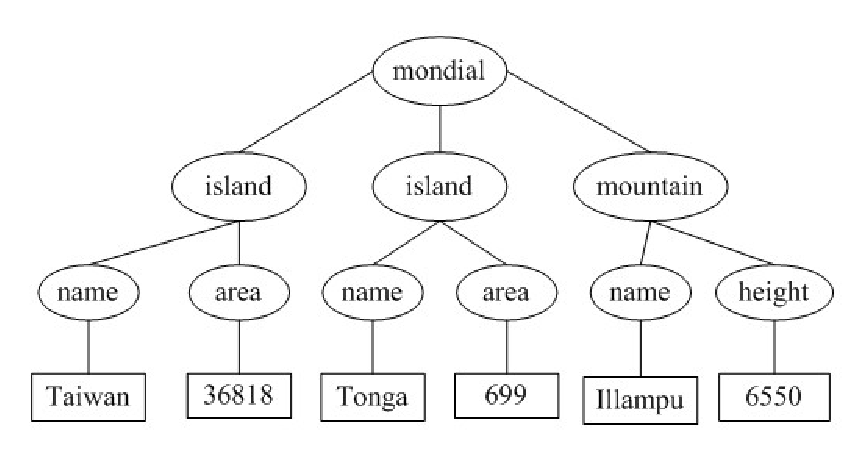
\includegraphics[width=0.4\textwidth]{XML}
\caption{树状结构}\label{fig:xml}
\vspace{\baselineskip}
\end{figure}


其插入图片的代码及其说明如下。
\vspace{1em}\noindent\hrule
\begin{verbatim}
\begin{figure}[htbp]
\centering
\includegraphics[width=0.4\textwidth]{文件名(.eps)}
\caption{标题}\label{标签名(通常为 fig:labelname)}
\vspace{\baselineskip} %表示图与正文空一行
\end{figure}
\end{verbatim}

\noindent\hrule

\begin{verbatim}
figure环境的可选参数[htbp]表示浮动图形所放置的位置,h (here)表示当前位置,t (top)表示页芯顶部,b (bottom)表示页芯底部,p (page)表示单独一页。在Word等软件中,图片通常插入到当前位置,如果当前页的剩余空间不够,图片将被移动到下一页,当前页就会出现很大的空白,其人工调整工作非常不便。由LaTeX提供的浮动图片功能,总是会按h->t->b->p的次序处理选项中的字母,自动调整图片的位置,大大减轻了工作量。
\centering命令将后续内容转换成每行皆居中的格式。
"\includegraphics"的可选参数用来设置图片插入文中的水平宽度,一般表示为正文宽度(\textwidth)的倍数。
\caption命令可选参数“标签名”为英文形式,一般不以图片或表格的数字顺序作为标签,而应包含一定的图片或表格信息,以便于文中引用(若图片、表格、公式、章节和参考文献等在文中出现的先后顺序发生了变化,其标注序号及其文中引用序号也会跟着发生变化,这一点是Word等软件所不能做到的)。另外,图题或表题并不会因为分页而与图片或表格体分置于两页,章节等各级标题也不会置于某页的最底部,LaTeX系统会自动调整它们在正文中的位置,这也是Word等软件所无法匹敌的。
\vspace将产生一定高度的竖直空白,必选参数为负值表示将后续文字位置向上提升,参数值可自行调整。em为长度单位,相当于大写字母M的宽度。\vspace{\baselineskip} 表示图与正文空一行。
引用方法:“见图~\ref{fig:figname}”、“如图~\ref{fig:figname}~所示”等。
\end{verbatim}

\noindent\hrule\vspace{1em}

若需要将~2~张及以上的图片并排插入到一行中,则需要采用\verb|minipage|环境,如图~\ref{fig:dd}~和图~\ref{fig:ds}~所示。
\begin{figure}[htbp]
\centering
\begin{minipage}{0.4\textwidth}
\centering
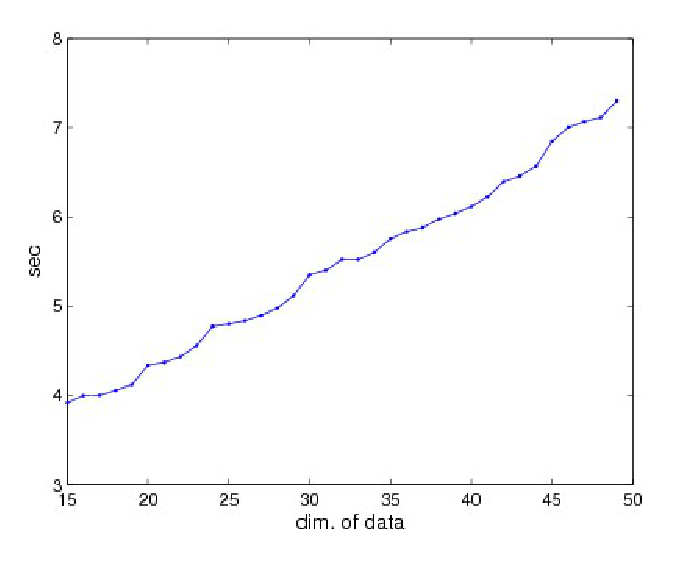
\includegraphics[width=\textwidth]{dataDimensions}
\caption{数据维数的变化}\label{fig:dd}
\end{minipage}
\begin{minipage}{0.4\textwidth}
\centering
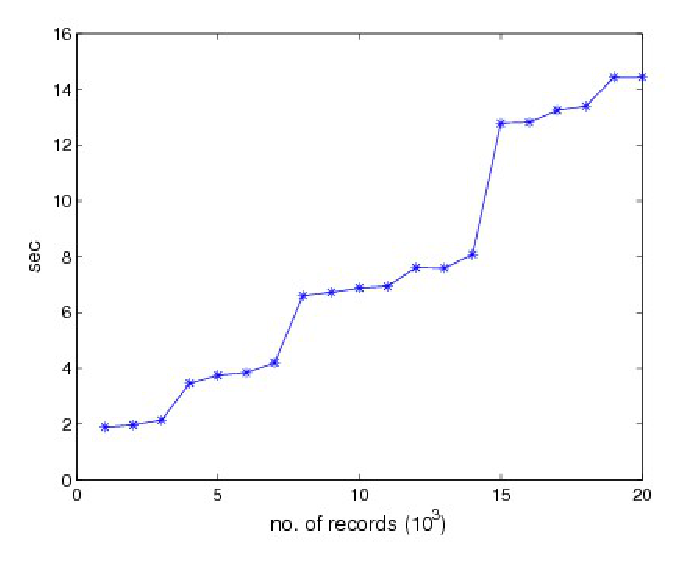
\includegraphics[width=\textwidth]{dataSize}
\caption{数据规模的变化}\label{fig:ds}
\end{minipage}
\vspace{\baselineskip}
\end{figure}

其代码如下所示。
\vspace{1em}\noindent\hrule
\begin{verbatim}
\begin{figure}[htbp]
\centering
\begin{minipage}{0.4\textwidth}
\centering
\includegraphics[width=\textwidth]{文件名}
\caption{标题}\label{fig:f1}
\end{minipage}
\begin{minipage}{0.4\textwidth}
\centering
\includegraphics[width=\textwidth]{文件名}
\caption{标题}\label{fig:f2}
\end{minipage}\vspace{\baselineskip}
\end{figure}
\end{verbatim}

\noindent\hrule

\begin{verbatim}
minipage环境的必选参数用来设置小页的宽度,若需要在一行中插入n个等宽图片,则每个小页的宽度应略小于(1/n)\textwidth。
\end{verbatim}

\noindent\hrule

\section{具有子图的图片插入方法}

图中若含有子图时,需要调用~subfigure~宏包, 如图~\ref{fig:subfig}~所示。
\begin{figure}[htbp]
  \centering
  \subfigure[Data Dimensions]{\label{fig:subfig:datadim}
                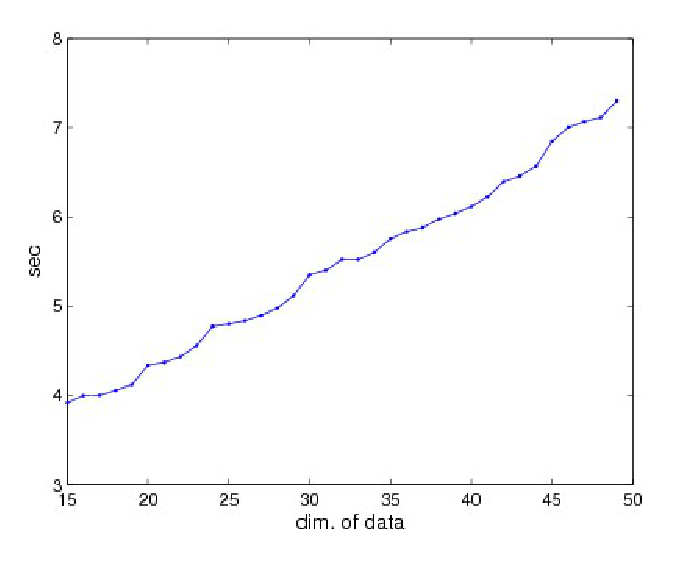
\includegraphics[width=0.4\textwidth]{dataDimensions}}
  \subfigure[Data Size]{\label{fig:subfig:datasize}
                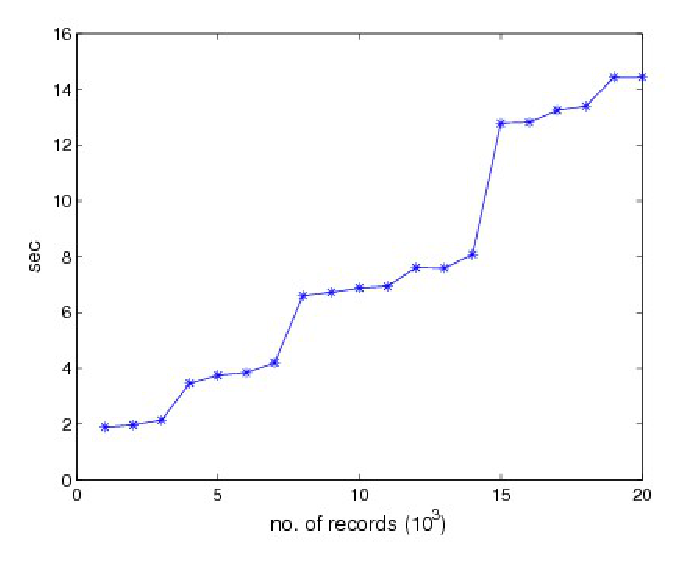
\includegraphics[width=0.4\textwidth]{dataSize}}
  \caption{Scalability of data}\label{fig:subfig}
\vspace{\baselineskip}
\end{figure}

其代码及其说明如下。
\vspace{1em}\noindent\hrule

\begin{verbatim}
\begin{figure}[htbp]
  \centering
  \subfigure[第1个子图标题]{
            \label{第1个子图标签(通常为 fig:subfig1:subsubfig1)}
            \includegraphics[width=0.4\textwidth]{文件名}}
  \subfigure[第2个子图标题]{
            \label{第2个子图标签(通常为 fig:subfig1:subsubfig2)}
            \includegraphics[width=0.4\textwidth]{文件名}}
  \caption{总标题}\label{总标签(通常为 fig:subfig1)}
\vspace{\baselineskip}
\end{figure}
\end{verbatim}

\noindent\hrule

\begin{verbatim}
子图的标签实际上可以随意设定,只要不重复就行。但为了更好的可读性,我们建议fig:subfig:subsubfig格式命名,这样我们从标签名就可以知道这是一个子图引用。
引用方法:总图的引用方法同本章第1节,子图的引用方法用\ref{fig:subfig:subsubfig}来代替。
\end{verbatim}

\noindent\hrule\vspace{1em}

子图的引用示例:如图~\ref{fig:subfig:datadim}~和图~\ref{fig:subfig:datasize}~所示。

若想获得插图方法的更多信息,参见网络上的~\href{ftp://ftp.tex.ac.uk/tex-archive/info/epslatex.pdf}{Using Imported Graphics in \LaTeX and pdf\LaTeX}~文档。 
%%% !Mode:: "TeX:UTF-8"

\chapter{表格的绘制方法}
\section{研究生毕业设计论文的绘表规范}

表应有自明性。表格不加左、右边线。表的编排建议采用国际通行的三线表。表内中文书写使用宋体五号字。

每个表格之上均应有表题(由表序和表名组成)。表序一般按章编排,如第~1~章第一个插表的序号为“表~1-1”等。表序与表名之间空两格,
表名使用中文五号字,居中。表名中不允许使用标点符号,表名后不加标点。
表头设计应简单明了,尽量不用斜线。表头中可采用化学,物理量等专业符号。

全表如用同一单位,则将单位符号移至表头右上角,加圆括号。
表中数据应准确无误,书写清楚。数字空缺的格内加横线“-”(占~2~个数字宽度)。表内文字或数字上、下或左、右相同时,
采用通栏处理方式,不允许用“〃”、“同上”之类的写法。

表内文字使用宋体五号字,垂直居中书写,起行空一格、转行顶格、句末不加标点。
如某个表需要转页接排,在随后的各页上应重复表的编号。编号后加“(续表)”,表题可省略。续表应重复表头。
表格绘制完成之后,与正文空一行。

\section{普通表格的绘制方法}

表格应具有三线表格式,因此需要调用~booktabs~宏包,其标准格式如表~\ref{tab:table1}~所示。
\begin{table}[htbp]
\caption{符合本科生毕业论文绘图规范的表格}\label{tab:table1}
\vspace{0.5em}\centering\wuhao
\begin{tabular}{ccccc}
\toprule[1.5pt]
$D$(in) & $P_u$(lbs) & $u_u$(in) & $\beta$ & $G_f$(psi.in)\\
\midrule[1pt]
 5 & 269.8 & 0.000674 & 1.79 & 0.04089\\
10 & 421.0 & 0.001035 & 3.59 & 0.04089\\
20 & 640.2 & 0.001565 & 7.18 & 0.04089\\
 5 & 269.8 & 0.000674 & 1.79 & 0.04089\\
10 & 421.0 & 0.001035 & 3.59 & 0.04089\\
20 & 640.2 & 0.001565 & 7.18 & 0.04089\\
 5 & 269.8 & 0.000674 & 1.79 & 0.04089\\
10 & 421.0 & 0.001035 & 3.59 & 0.04089\\
20 & 640.2 & 0.001565 & 7.18 & 0.04089\\
 5 & 269.8 & 0.000674 & 1.79 & 0.04089\\
10 & 421.0 & 0.001035 & 3.59 & 0.04089\\
20 & 640.2 & 0.001565 & 7.18 & 0.04089\\
\bottomrule[1.5pt]
\end{tabular}
\vspace{\baselineskip}
\end{table}

其绘制表格的代码及其说明如下。
\vspace{1em}\noindent\hrule

\begin{verbatim}
\begin{table}[htbp]
\caption{表标题}\label{标签名(通常为 tab:tablename)}
\vspace{0.5em}\centering\wuhao
\begin{tabular}{cc...c}
\toprule[1.5pt]
表头第1个格   & 表头第2个格   & ... & 表头第n个格  \\
\midrule[1pt]
表中数据(1,1) & 表中数据(1,2) & ... & 表中数据(1,n)\\
表中数据(2,1) & 表中数据(2,2) & ... & 表中数据(2,n)\\
表中数据(3,1) & 表中数据(3,2) & ... & 表中数据(3,n)\\
表中数据(4,1) & 表中数据(4,2) & ... & 表中数据(4,n)\\
...................................................\\
表中数据(m,1) & 表中数据(m,2) & ... & 表中数据(m,n)\\
\bottomrule[1.5pt]
\end{tabular}
\vspace{\baselineskip}
\end{table}
\end{verbatim}

\noindent\hrule

\begin{verbatim}
table环境是一个将表格嵌入文本的浮动环境。
\wuhao命令将表格的字号设置为五号字(10.5pt),在绘制表格结束退出时,不需要将字号再改回为\xiaosi,正文字号默认为小四号字(12pt)。
tabular环境的必选参数由每列对应一个格式字符所组成:c表示居中,l表示左对齐,r表示右对齐,其总个数应与表的列数相同。此外,@{文本}可以出现在任意两个上述的列格式之间,其中的文本将被插入每一行的同一位置。表格的各行以\\分隔,同一行的各列则以&分隔。
\toprule、\midrule和\bottomrule三个命令是由booktabs宏包提供的,其中\toprule和\bottomrule分别用来绘制表格的第一条(表格最顶部)和第三条(表格最底部)水平线,\midrule用来绘制第二条(表头之下)水平线,且第一条和第三条水平线的线宽为1.5pt,第二条水平线的线宽为1pt。
引用方法:“如表~\ref{tab:tablename}~所示”。
\end{verbatim}

\noindent\hrule

\section{长表格的绘制方法}

长表格是当表格在当前页排不下而需要转页接排的情况下所采用的一种表格环境。若长表格仍按照普通表格的绘制方法来获得,
其所使用的\verb|table|浮动环境无法实现表格的换页接排功能,表格下方过长部分会排在表格第1页的页脚以下。为了能够实现长表格的转页接排功能,
需要调用~longtable~宏包,由于长表格是跨页的文本内容,因此只需要单独的\verb|longtable|环境,所绘制的长表格的格式如表~\ref{tab:table2}~所示。

此长表格~\ref{tab:table2}~第~2~页的标题“编号(续表)”和表头是通过代码自动添加上去的,无需人工添加,若表格在页面中的竖直位置发生了变化,长表格在第~2~页
及之后各页的标题和表头位置能够始终处于各页的最顶部,也无需人工调整,\LaTeX~系统的这一优点是~Word~等软件所无法企及的。

下段内容是为了让下面的长表格分居两页,看到表标题“编号(续表)”的效果。摘录于《你若安好,便是晴天 -- 林徽因传》片段:

她叫林徽因,出生于杭州,是许多人梦中期待的白莲。她在雨雾之都伦敦,发生过一场空前绝后的康桥之恋。她爱过三个男子,爱得清醒,也爱得平静。徐志摩为她徜徉在康桥,深情地等待一场旧梦可以归来。梁思成与她携手走过千山万水,为完成使命而相约白头。金岳霖为她终身不娶,痴心不改地守候一世。可她懂得人生飘忽不定,要学会随遇而安。
真正的平静,不是避开车马喧嚣,而是在心中修篱种菊。尽管如流往事,每一天都涛声依旧,只要我们消除执念,便可寂静安然。愿每个人在纷呈世相中不会迷失荒径,可以端坐磐石上,醉倒落花前。
如果可以,请让我预支一段如莲的时光,哪怕将来某一天加倍偿还。这个雨季会在何时停歇,无从知晓。但我知道,你若安好,便是晴天。					
\wuhao\begin{longtable}{ccc}
\caption{天津大学各学院名称一览}\label{tab:table2}
 \vspace{0.5em}\\
\toprule[1.5pt] 学院名称 & 网址 & 联系电话  \\ \midrule[1pt]
\endfirsthead
\multicolumn{3}{c}{表~\thetable(续表)}\vspace{0.5em}\\
\toprule[1.5pt] 学院名称 & 网址 & 联系电话  \\ \midrule[1pt]
\endhead
\bottomrule[1.5pt]
\endfoot
机械工程学院& \url{http://tdjxxy.tju.edu.cn/}& 87401979\\
精密仪器与光电子工程学院&  \url{http://www2.tju.edu.cn/colleges/precision/cn/}& 27404775\\
电子信息工程学院& \url{http://www.tju.edu.cn/seie}& 27406956\\
电气与自动化工程学院& \url{http://www2.tju.edu.cn/colleges/automate/}& 27405477\\
建筑工程学院& \url{http://www2.tju.edu.cn/colleges/civil/}& 27404072\\
化工学院& \url{http://chemeng.tju.edu.cn/}& 27403389\\
材料科学与工程学院& \url{http://mse.tju.edu.cn}& 27406693 \\
建筑学院& \url{http://hgw022072.chinaw3.com/}& 27402724-2111\\
求是学部\\
管理与经济学部&	\url{ http://sm.tju.edu.cn}& 27403423\\
理学院& \url{ http://www.tju.edu.cn/science/}& 27404118\\
文法学院& \url{ http://www2.tju.edu.cn/colleges/sociology/new/}& 27403691\\
软件学院& \url{http://scs.tju.edu.cn}& 87401540\\
计算机科学与技术学院& \url{http://cs.tju.edu.cn/}& 27406538\\
马克思主义学院& \url{http://www2.tju.edu.cn/colleges/marxism/}& 27405348\\
环境科学与工程学院& \url{http://www.tju.edu.cn/see}& 87402072\\
药物科学与技术学院& \url{http://www2.tju.edu.cn/colleges/pharmtier/}& 87401830\\
教育学院& \url{http://soe.tju.edu.cn/}& 27401028\\
职业技术教育学院& \url{http://202.113.0.248:8888}\\
继续教育学院& \url{http://aectu.tju.edu.cn/}& 27406298\\
仁爱学院& \url{http://www.tjrac.edu.cn/}& 68579990\\
农业与生物工程学院& \url{http://202.113.13.169/site/nongxueyuan/}& 87402171\\
国际教育学院 & \url{http://www.ietju.com/}& 27406147\\
网络教育学院 & \url{http://www.etju.com/}& 27426952 \\

\end{longtable}\xiaosi
\vspace{\baselineskip}

绘制长表格的代码及其说明如下。
\vspace{1em}\noindent\hrule

\begin{verbatim}
\wuhao\begin{longtable}{cc...c}
\caption{表标题}\label{标签名(通常为 tab:tablename)}\\
\toprule[1.5pt] 表头第1个格 & 表头第2个格 & ... & 表头第n个格\\ \midrule[1pt]
\endfirsthead
\multicolumn{n}{c}{表~\thetable(续表)}\vspace{0.5em}\\
\toprule[1.5pt] 表头第1个格 & 表头第2个格 & ... & 表头第n个格\\ \midrule[1pt]
\endhead
\bottomrule[1.5pt]
\endfoot
表中数据(1,1) & 表中数据(1,2) & ... & 表中数据(1,n)\\
表中数据(2,1) & 表中数据(2,2) & ... & 表中数据(2,n)\\
...................................................\\
表中数据(m,1) & 表中数据(m,2) & ... & 表中数据(m,n)\\
\end{longtable}\xiaosi
\end{verbatim}

\noindent\hrule
\begin{verbatim}
在绘制长表格的前面留出一个空白行,并在第2行的一开始全局定义长表格的字号为五号字,这样能够保证长表格之前段落的行距保持不变。
在绘制长表格结束后,需要\xiaosi命令重新将字号改为小四号字。
\endhead之前的文字描述的是第2页及其之后各页的标题或表头;
\endfirsthead之前的文字描述的是第1页的标题和表头,若无此命令,则第1页的表头和标题由\endhead命令确定;
同理,\endfoot之前的文字描述的是除最后一页之外每页的表格底部内容;
\endlastfoot之前的文字描述的是最后一页的表格底部内容,若无此命令,
则最后一页的表格底部内容由\endfoot命令确定;由于规范中长表格每页底部内容均相同(水平粗线),因此模板中没有用到\endlastfoot命令。
\end{verbatim}

\noindent\hrule
\section{列宽可调表格的绘制方法}
论文中能用到列宽可调表格的情况共有两种:一种是当插入的表格某一单元格内容过长以至于一行放不下的情况,
另一种是当对公式中首次出现的物理量符号进行注释的情况。这两种情况都需要调用~tabularx~宏包。下面将分别对这两种情况下可调表格的绘制方法进行阐述。
\subsection{表格内某单元格内容过长的情况}

首先给出这种情况下的一个例子如表~\ref{tab:table3}~所示。
\begin{table}[htbp]
\caption{最小的三个正整数的英文表示法}\label{tab:table3}
\vspace{0.5em}\wuhao
\begin{tabularx}{\textwidth}{llX}
\toprule[1.5pt]
Value & Name & Alternate names, and names for sets of the given size\\\midrule[1pt]
1 & One & ace, single, singleton, unary, unit, unity\\
2 & Two & binary, brace, couple, couplet, distich, deuce, double, doubleton, duad, duality, duet, duo, dyad, pair, snake eyes, span, twain, twosome, yoke\\
3 & Three & deuce-ace, leash, set, tercet, ternary, ternion, terzetto, threesome, tierce, trey, triad, trine, trinity, trio, triplet, troika, hat-trick\\\bottomrule[1.5pt]
\end{tabularx}
\vspace{\baselineskip}
\end{table}
绘制这种表格的代码及其说明如下。
\vspace{1em}\noindent\hrule
\begin{verbatim}
\begin{table}[htbp]
\caption{表标题}\label{标签名(通常为 tab:tablename)}
\vspace{0.5em}\wuhao
\begin{tabularx}{\textwidth}{l...X...l}
\toprule[1.5pt]
表头第1个格   & ... & 表头第X个格   & ... & 表头第n个格  \\
\midrule[1pt]
表中数据(1,1) & ... & 表中数据(1,X) & ... & 表中数据(1,n)\\
表中数据(2,1) & ... & 表中数据(2,X) & ... & 表中数据(2,n)\\
.........................................................\\
表中数据(m,1) & ... & 表中数据(m,X) & ... & 表中数据(m,n)\\
\bottomrule[1.5pt]
\end{tabularx}
\vspace{\baselineskip}
\end{table}
\end{verbatim}

\noindent\hrule
\begin{verbatim}
tabularx环境共有两个必选参数:第1个参数用来确定表格的总宽度,这里取为排版表格能达到的最大宽度——正文宽度\textwidth;第2个参数用来确定每列格式,其中标为X的项表示该列的宽度可调,其宽度值由表格总宽度确定。
标为X的列一般选为单元格内容过长而无法置于一行的列,这样使得该列内容能够根据表格总宽度自动分行。若列格式中存在不止一个X项,则这些标为X的列的列宽相同,因此,一般不将内容较短的列设为X。
标为X的列均为左对齐,因此其余列一般选为l(左对齐),这样可使得表格美观,但也可以选为c或r。
\end{verbatim}

\noindent\hrule
\subsection{对物理量符号进行注释的情况}
为使得对公式中物理量符号注释的转行与破折号“———”后第一个字对齐,此处最好采用表格环境。此表格无任何线条,左对齐,
且在破折号处对齐,一共有“式中”二字、物理量符号和注释三列,表格的总宽度可选为文本宽度,因此应该采用\verb|tabularx|环境。
由\verb|tabularx|环境生成的对公式中物理量符号进行注释的公式如式(\ref{eq:1})所示。
%\vspace*{10pt}

\begin{equation}\label{eq:1}
\ddot{\boldsymbol{\rho}}-\frac{\mu}{R_{t}^{3}}\left(3\mathbf{R_{t}}\frac{\mathbf{R_{t}\rho}}{R_{t}^{2}}-\boldsymbol{\rho}\right)=\mathbf{a}
\end{equation}

\begin{tabularx}{\textwidth}{@{}l@{\quad}r@{———}X@{}}
式中& $\bm{\rho}$ &追踪飞行器与目标飞行器之间的相对位置矢量;\\
&  $\bm{\ddot{\rho}}$&追踪飞行器与目标飞行器之间的相对加速度;\\
&  $\mathbf{a}$   &推力所产生的加速度;\\
&  $\mathbf{R_t}$ & 目标飞行器在惯性坐标系中的位置矢量;\\
&  $\omega_{t}$ & 目标飞行器的轨道角速度;\\
&  $\mathbf{g}$ & 重力加速度,$=\frac{\mu}{R_{t}^{3}}\left(
3\mathbf{R_{t}}\frac{\mathbf{R_{t}\rho}}{R_{t}^{2}}-\bm{\rho}\right)=\omega_{t}^{2}\frac{R_{t}}{p}\left(
3\mathbf{R_{t}}\frac{\mathbf{R_{t}\rho}}{R_{t}^{2}}-\bm{\rho}\right)$,这里~$p$~是目标飞行器的轨道半通径。
\end{tabularx}
\vspace{\wordsep}

其中生成注释部分的代码及其说明如下。

\vspace{1em}\noindent\hrule

\begin{verbatim}
\begin{tabularx}{\textwidth}{@{}l@{\quad}r@{— — —}X@{}}
式中 & symbol-1 & symbol-1的注释内容;\\
     & symbol-2 & symbol-2的注释内容;\\
     .............................;\\
     & symbol-m & symbol-m的注释内容。
\end{tabularx}\vspace{\wordsep}
\end{verbatim}

\noindent\hrule

\begin{verbatim}
tabularx环境的第1个参数选为正文宽度,第2个参数里面各个符号的意义为:
    第1个@{}表示在“式中”二字左侧不插入任何文本,“式中”二字能够在正文中左对齐,若无此项,则“式中”二字左侧会留出一定的空白;
    @{\quad}表示在“式中”和物理量符号间插入一个空铅宽度的空白;
    @{— — —}实现插入破折号的功能,它由三个1/2的中文破折号构成;
    第2个@{}表示在注释内容靠近正文右边界的地方能够实现右对齐。
\end{verbatim}

\noindent\hrule\vspace{1em}

由此方法生成的注释内容应紧邻待注释公式并置于其下方,因此不能将代码放入\verb|table|浮动环境中。但此方法不能实现自动转页接排,
可能会在当前页剩余空间不够时,全部移动到下一页而导致当前页出现很大空白。因此在需要转页处理时,还请您手动将需要转页的代码放入一个
新的\verb|tabularx|环境中,将原来的一个\verb|tabularx|环境拆分为两个\verb|tabularx|环境。

若想获得绘制表格的更多信息,参见网络上的~\href{http://www.tug.org/pracjourn/2007-1/mori/}{Tables in \LaTeXe: Packages and Methods}~文档。


%%\include{body/equations}
%%% !Mode:: "TeX:UTF-8"

\chapter{罗列和定理环境使用方法}

\section{单层罗列环境}
天津大学学位论文一般可采用两种罗列环境:一种是并列条目有同样标签的~\verb|itemize|~罗列环境,另一种是具有自动排序编号符号的~\verb|enumerate|~罗列环境。这两种罗列环境的样式参数可参考图~\ref{fig:list}。
\begin{figure}[htbp]
\centering
\includegraphics[width = 0.6\textwidth]{list}
\caption{罗列环境参数示意图}\label{fig:list}\vspace{-1em}
\end{figure}

通过调用~enumitem~宏包可以很方便地控制罗列环境的布局,其~format.tex~文件中的~\verb|\setitemize|~和~\verb|\setenumerate|~命令分别用来设置~\verb|itemize|~和~\verb|enumerate|~环境的样式参数。采用~\verb|itemize|~单层罗列环境的排版形式如下:

\begin{itemize}
\item 第一个条目文本内容
\item 第二个条目文本内容
\item 第三个条目文本内容
\end{itemize}

其代码如下

\begin{verbatim}
\begin{itemize}
  \item 第一个条目文本内容
  \item 第二个条目文本内容
  ...
  \item 第三个条目文本内容
\end{itemize}
\end{verbatim}

采用~\verb|enumerate|~单层罗列环境的排版形式如下:

\begin{enumerate}
\item 第一个条目文本内容
\item 第二个条目文本内容
\item 第三个条目文本内容
\end{enumerate}

其代码如下

\begin{verbatim}
\begin{enumerate}
  \item 第一个条目文本内容
  \item 第二个条目文本内容
  ...
  \item 第三个条目文本内容
\end{enumerate}
\end{verbatim}



\section{定理环境}

\begin{definition}[谱半径]\label{def:def1}
  称~$n$~阶方阵~$\mathbf{A}$~的全体特征值~$\lambda_1,\cdots,\lambda_n$~组成的集合为~$\mathbf{A}$~的谱,称
  $$\rho(\mathbf{A})=\max{\{|\lambda_1|,\cdots,|\lambda_n|\}}$$
\end{definition}
\begin{theorem}[相似充要条件]\label{lemma:l1}
  方阵$A$和$B$相似的充要条件是:~$A$~和~$B$~有全同的不变因子。
\end{theorem}
\begin{corollary}[推论1]\label{cor:cor1}
在赋范空间~$(X,\|\cdot\|)$~上定义~$d(x,y)=\|x-y\|$, 对任意~$x,y\in X$,~则~$(X,d)$~是距离空间。
\end{corollary}
\begin{proof}
  只需证明~$d(x,y)$~是距离。
\end{proof}
\newpage

定义代码如下:
\begin{verbatim}
 \begin{definition}[谱半径]\label{def:def1}
  称~$n$~阶方阵~$\mathbf{A}$~的全体特征值
  $\lambda_1,\cdots,\lambda_n$组成的集合为~$\mathbf{A}$~的谱,称
  $$\rho(\mathbf{A})=\max{\{|\lambda_1|,\cdots,|\lambda_n|\}}$$
\end{definition}
\end{verbatim}
\noindent\hrule

\vspace{0.1em}\noindent\hrule
\vspace{1em}
定理代码如下:
\begin{verbatim}
\begin{theorem}[相似充要条件]\label{lemma:l1}
  方阵$A$和$B$相似的充要条件是:$A$和$B$有全同的不变因子。
\end{theorem}
\end{verbatim}
\noindent\hrule\vspace{0.1em}

\noindent\hrule
\vspace{1em}
推论和证明代码如下:
\begin{verbatim}
\begin{corollary}[推论1]\label{cor:cor1}
在赋范空间~$(X,\|\cdot\|)$~上定义$d(x,y)=\|x-y\|$,
对任意$x,y\in X$,则$(X,d)$是距离空间。
\end{corollary}
\begin{proof}
  只需证明$d(x,y)$是距离。
\end{proof}
\end{verbatim}
\noindent\hrule\vspace{1em}

定理定义[]中是可选参数,用来说明定理的名称。其他环境格式书写与上面定理、定义、推论格式相同,可自己调用其他环境。
若需要书写定理定义等内容,而且带有顺序编号,需要采用如下环境。除了~\verb|proof|~环境之外,其余~9~个环境都可以有一个可选参数作为附加标题。

\begin{center}
\vspace{0.5em}\noindent\wuhao\begin{tabularx}{0.7\textwidth}{lX|lX}
定理 & \verb|theorem|~环境 & 定义 & \verb|definition|~环境 \\
例 & \verb|example|~环境 & 算法 & \verb|algorithm|~环境 \\
公理 & \verb|axiom|~环境 & 命题 & \verb|proposition|~环境 \\
引理 & \verb|lemma|~环境 & 推论 & \verb|corollary|~环境 \\
注解 & \verb|remark|~环境 & 证明 & \verb|proof|~环境 \\
\end{tabularx}
\end{center} 
%%\include{body/conclusion}
\end{verbatim}
那么,编译的时候就只编译未加~\%~的一章,在这个例子中,即本章~intros。

理论上,并不一定要把每章放在不同的文件中。但是这种自顶向下,分章节写作、编译的方法有利于提高效率,大大减少~Debug~过程中的编译时间,同时减小风险。

\section{参考文献生成方法}

\LaTeX~具有插入参考文献的能力。Google Scholar~网站上存在兼容~BibTeX~的参考文献信息,通过以下几个步骤,可以轻松完成参考文献的生成。
\begin{itemize}
  \item 在\href{http://scholar.google.com/}{谷歌学术搜索}中,
        点击\href{http://scholar.google.com/scholar_preferences?hl=en&as_sdt=0,5}{学术搜索设置}。
  \item 页面打开之后,在\textbf{文献管理软件}选项中选择\textbf{显示导入~BibTeX~的链接},单击保存设置,退出。
  \item 在谷歌学术搜索中检索到文献后,在文献条目区域单击导入~BibTeX~选项,页面中出现文献的引用信息。
  \item 将文献引用信息的内容复制之后,添加到~references~文件夹下的~reference.bib~中。
\end{itemize}

\section{编译注意事项}
\begin{enumerate}
  \item 由于模板使用~UTF-8~编码,所以源文件应该保存成~UTF-8~格式,否则可能出现中文字符无法识别的错误。
  本模板中每一个~.tex~文件的文件的开头已经加上一行:\\
    \verb|% !Mode:: "TeX:UTF-8"|\\
     这样可以确保~.tex~文件默认使用~UTF-8~的格式打开。读者如果删去此行,很有可能会导致中文字符显示乱码。
     在~WinEdt~编辑器中可以使用以下两种方式保存成~UTF-8~格式:
      \begin{enumerate}
        \item 先建立~.tex~文件,另存为~.tex~文件时,选择用~UTF-8~格式保存。
        \item
            在~WinEdt~编辑器中,选择\\
            \mbox{~Document$\to$Document Settings$\to$Document Mode $\to$TeX:UTF-8} 同时在~WinEdt~最下面的状态栏中,可以看到该文档是~TeX~格式还是~TeX:UTF-8~格式。
            当文档为~TeX:UTF-8~格式时,状态栏一般显示:
            \makebox[\textwidth][l]{Wrap | Indent | INS | LINE |Spell | TeX:UTF-8 | -src~等。}
      \end{enumerate}
  \item 如果在pdf书签中,中文显示乱码的话,则注意以下说明:
    \begin{verbatim}
        \usepackage{CJKutf8}
        % 1. 如果使用CJKutf8
        %    Hyperref中应使用unicode参数
        % 2. 如果使用CJK
        %    Hyperref则使用CJKbookmarks参数
        %    可惜得到的PDF书签是乱码,建议弃用
        % 3. Unicode选项和CJKbookmarks不能同时使用
        \usepackage[
        %CJKbookmarks=true,
        unicode=true
        ]{hyperref}
     \end{verbatim}
 \item 建议采用以下两种编译方式:
  \begin{enumerate}
     \item latex + bibtex + latex + latex + dvi2pdf. 在这种编译情况下,对应的~tjumain.tex~文件的第一行是\verb|\def\usewhat{dvipdfmx}|~(缺省设置)。 此时,所有图片文件应该保存为~.eps~格式,如~figures~文件夹里~.eps~图片。
          如果您选择在命令行中操作,可以在编译的时候依次输入~latex tjumain, bibtex tjumain, latex tjumain, latex tjumain~和~dvipdfmx tjumain, 编译完成之后,需要手动打开~pdf~文件。
     \item pdflatex + pdflatex. 在这种编译情况下,对应的~tjumain.tex~文件的第一行应该改为\verb|\def\usewhat{pdflatex}|~。 此时, 编译不支持~.eps~图片格式,此时需要在命令行下使用~epstopdf~指令将~figures~文件夹下 的~.eps~文件转化成~.pdf~文件格式,命令行中操作格式为~epstopdf a.eps~。
          在命令行编译的时候,依次输入~pdflatex tjumain~和~pdflatex tjumain, 编译完成之后,需要手动打开~pdf~文件。
  \end{enumerate}
\end{enumerate}

\section{系统要求}
    CTEX 2.8, MiKTeX 2.8, TeX Live 2009~或以上版本。使用推荐的~WinEdt 6.0~编辑器,可以完成文件的编辑和编译工作。

\section{\TeX~简介}

以下内容是~milksea@bbs.ctex.org~撰写的关于~\TeX~的简单介绍,略有改动。
注意这不是一个入门教程,不讲~\TeX~系统的配置安装,也不讲具体的~\LaTeX~代码。
这里仅仅试图以一些只言片语来解释:
进入这个门槛之前新手应该知道的注意事项,以及遇到问题以后该去如何解决问题。

\subsection{什么是 \TeX/\LaTeX,我是否应该选择它~?}

\TeX~是最早由高德纳(Donald Knuth)教授创建的一门标记式宏语言,
用来排版科技文章,尤其擅长处理复杂的数学公式。\TeX~同时也是处理这一语言的排版软件。
\LaTeX~是 Leslie Lamport 在~\TeX~基础上按内容/格式分离和模块化等思想建立的一集~\TeX~上的格式。

\TeX~本身的领域是专业排版领域
但现在~TeX/LaTeX~也被广泛用于生成电子文档甚至幻灯片等,~\TeX~语言的数学部分
偶尔也在其他一些地方使用。但注意~\TeX~并不适用于文书处理(Microsoft Office 的领域,以前和现在都不是)。

选择使用~\TeX/\LaTeX~的理由包括:
\begin{itemize}
\item 免费软件;
\item 专业的排版效果;
\item 是事实上的专业数学排版标准;
\item 广泛的西文期刊接收甚或只接收 LaTeX 格式的投稿;
\item[] ……
\end{itemize}
不选择使用~\TeX/\LaTeX~的理由包括:
\begin{itemize}
\item 需要相当精力学习;
\item 图文混合排版能力不够强;
\item 仅在数学、物理、计算机等领域流行;
\item 中文期刊的支持较差;
\item[] ……
\end{itemize}

请尽量清醒看待网上经常见到的关于~\TeX~与其他软件的优劣比较和口水战。在选择使用或离开之前,请先考虑
\TeX~的应用领域,想想它是否适合你的需要。


\subsection{我该用什么编辑器~?}

编辑器功能有简有繁,特色不一,从简单的纯文本编辑器到繁复的 Emacs,因人而易。基本功能有语法高亮、方便编译预览就很好了,扩充功能和定制有无限的可能。初学者可以使用功能简单、使用方便的专用编辑器,如 ~TeXWorks、Kile、WinEdt~等,或者类似所见即所得功能的~LyX;熟悉的人可以使用定制性更强的~Notepad++、SciTE、Vim、Emacs ~等。这方面的介绍很多,一开始不妨多试几种,找到最适合自己的才是最好的。

另外提醒一句,编辑器只是工作的助手,不必把它看得太重。

\subsection{我应该看什么~\LaTeX~读物~?}

这不是一个容易回答的问题,因为有许多选择,也同样有许多不合适的选择。
这里只是选出一个比较好的答案。更多更详细的介绍可以在版面和网上寻找(注意时效)。

近两年~\TeX~的中文处理发展很快,目前没有哪本书在中文处理方面给出一个最新进展的合适综述,
因而下面的介绍也不主要考虑中文处理。

\begin{enumerate}

\item 我能阅读英文。
\begin{enumerate}
\item 迅速入门:ltxprimer.pdf (LaTeX Tutorials: A Primer, India TUG)
\item 系统学习:A Guide to LaTeX, 4th Edition, Addison-Wesley
               有机械工业出版社的影印版(《\LaTeX{}~实用教程》)
\item 深入学习:要读许多书和文档,TeXbook 是必读的
\item 细节学习:去读你使用的每一个宏包的说明文档
\item 专题学习:阅读讲数学公式、图形、表格、字体等的专题文档
\end{enumerate}

\item 我更愿意阅读中文。
\begin{enumerate}
\item 迅速入门:lnotes.pdf (LaTeX Notes, 1.20, Alpha Huang)
\item 系统学习:《\LaTeXe{}~科技排版指南》,邓建松(电子版)
      如果不好找,可以阅读《\LaTeXe~入门与提高》第二版,陈志杰等,或者 《\LaTeXe~完全学习手册》,胡伟
\item 深入学习:~TeXbook0.pdf~(特可爱原本,TeXbook 的中译,xianxian)
\item 具体问题释疑:~CTeX-FAQ.pdf~,\\
        吴凌云,~\url{http://www.ctex.org/CTeXFAQ}~
\end{enumerate}
\end{enumerate}

遇见问题和解决问题的过程可以快速提高自己的技能,建议此时:
\begin{itemize}
  \item 利用~Google~搜索。
  \item 清楚,扼要地提出你的问题。
\end{itemize}

\subsection{什么知识会过时~?什么不会~?}

\TeX~是排版语言,也是广泛使用的软件,并且不断在发展中;
因此,总有一些东西会很快过时。作为学习~\TeX~的人,
免不了要看各种各样的书籍、电子文档和网络论坛上的只言片语,
因此了解什么知识会迅速过时,什么知识不会是十分重要的。

最稳定的是关于~Primitive \TeX~和~Plain \TeX~的知识,也就是 Knuth
在他的《The TeXbook》中介绍的内容。因为~\TeX~
系统开发的初衷就是稳定性,要求今天的文档到很久以后仍可以得到完全相同的结果,
因此 Knuth 限定了他的~\TeX~语言和相关实现的命令、语法。这些内容许多年来就没有多少变化,
在未来的一些年里也不会有什么变化。
Primitive \TeX~和 Plain \TeX~的知识主要包括 \TeX~排版的基本算法和原理,
盒子的原理,底层的 \TeX~命令等。其中技巧性的东西大多在宏包设计中,
初学者一般不会接触到很多;而基本原理则是常常被提到的,
譬如,~\TeX~把一切排版内容作为盒子(box)处理。

相对稳定的是关于基本~\LaTeXe~
的知识,也包括围绕~\LaTeXe~的一些核心宏包的知识。~\LaTeXe~
是自~1993~年以来的一个稳定的~\LaTeX~版本,直到最近的一次修订
(2005 年)都没有大的变动。
\LaTeX~的下一个计划中的版本~\LaTeX 3~遥遥无期,在可预见的将来,~\LaTeXe~不会过时。
\LaTeXe~的知识是目前大部分~\LaTeX~书籍的主体内容。关于~\LaTeX~的标准文档类
~(article、report、book、letter、slide~等),关于基本数学公式的输入,
文档的章节层次,表格和矩阵,图表浮动体,LR 盒子与段落盒子……
这些~\LaTeX~的核心内容都是最常用的,相对稳定的。
与~\LaTeXe~相匹配的核心宏包,
如~graphics(x)、ifthen、fontenc、doc~等,也同样是相对稳定的。
还有一些被非常广泛应用的宏包,如~amsmath~系列,也可以看作是相对稳定的。

简单地说,关于基本~\TeX/\LaTeX~的语言,都是比较稳定的。与之对应,实现或者支持~\TeX/\LaTeX~语言的软件,
包括在~\TeX/\LaTeX~基础上建立的新的宏,都不大稳定。

容易过时的是关于第三方~\LaTeX~宏包的知识、第三方~\TeX~工具的知识,以及新兴~\TeX~相关软件的知识等。
~\TeX~和~\LaTeX~语言是追求稳定的;但无论是宏包还是工具,作为不断更新软件,它们是不稳定的。
容易过时的技术很多,而且现在广泛地出现在几乎所有~\LaTeX~文档之中,因此需要特别引起注意:
宏包的过时的原因可能是宏包本身的升级换代带来了新功能或不兼容,
也可能是同一功能的更新更好的宏包代替了旧的宏包。前者的典型例子比如绘图宏包~PGF/TikZ~,
现在的~2.00~版功能十分强大,和旧的~1.1x~版相差很大,和更旧的~0.x~版本则几乎完全不同;后
者的典型例子比如~caption~宏包先是被更新的~caption2~宏包代替,后来~caption~宏包更新又使得
caption2 宏包完全过时。——安装更新的发行版可以避免使用过旧的宏包;
认真阅读宏包自带的文档而不是搜索得到的陈旧片断可以避免采用过时的代码。

工具过时的主要原因也是升级换代和被其他工具替换。前者的典型例子是编辑器
WinEdt~在~5.5~以后的版本支持~UTF-8~编码,而旧版本不支持;
后者的典型例子是中文字体安装工具从~GBKFonts~到~xGBKFonts~到~FontsGen~不断被取代。
图形插入是一个在~\TeX~实现、宏包与外围工具方面都更新很快的东西。
在过去,最常用的输出格式是~PS(PostScript)~格式,因此插入的图像以~EPS~为主流。
使用~Dvips~为主要输出工具,外围工具有~GhostScript、bmeps~等等,相关宏包有~graphics~等,
相关文档如《\LaTeXe{}~ 插图指南》。

但凡提及“~\LaTeX~只支持~EPS~图形”的,就是这个过时的时代的产物。事实上~\TeX/\LaTeX~
并不限定任何图形格式,只不过是当时的输出格式(PS)和工具(Dvips)对~EPS~情有独钟而已。
后来 PDF 格式成为主流。~pdf\TeX、DVIPDFM、DVIPDFMx、XeTeX~工具则主要支持~PDF、PNG、JPG~格式的图形,
涉及一系列工具如~ImageMagick、ebb~等。

值得特别提出注意的就是,中文处理也一起是更新迅速、容易过时的部分。
而且因为中文处理一直没有一个“官方”的“标准”做法,软件、工具、
文档以及网上纷繁的笔记也就显得相当混乱。从八十年代开始的~CCT~系统、
天元系统,到后来的~CJK~方式,到近来的~XeTeX~和~LuaTeX~ 方式,
中文处理的原理、软件、宏包、配置方式等都在不断变化中。

\section{后期工作}
下表记录了~TJUThesis~计划中未来应该逐步实现的功能和特性:
\begin{enumerate}
  \item 编写更为详细的~TJUThesis~的使用手册和~FAQ~用户指南
  \item 加入对课程结课论文的支持
  \item 加入对天津大学学生经常参加的各种限时完成重大赛事的论文模板的支持,如全国研究生数学建模竞赛,以节省排版时间
  \item 加入对~pdf~书签中章节中文编号的支持,如: 第一章 XXX
  \item 加入对附录~A~等格式的支持
  \item Linux~平台迁移和测试
\end{enumerate}

\section{免责声明}

本模板依据《天津大学关于博士、硕士学位论文统一格式的规定》和《天津大学硕士论文模版》编写,适用于所有硕士生的学位论文编写。然而,作者不保证本模板完全符合学校要求,也不对由此带来的风险和损失承担任何责任。

% !Mode:: "TeX:UTF-8"

\chapter{图片的插入方法}

\section{博士学位论文的插图规范}

图应有自明性。插图应与文字紧密配合,文图相符,内容正确。选图要力求精练,插图、照片应完整清晰。图中文字和数字等字号用宋体五号字。

机械工程图:采用第一角投影法,严格按照~GB4457---GB131-83《机械制图》标准规定。

数据流程图、程序流程图、系统流程图等按~GB1526-89~标准规定。

电气图:图形符号、文字符号等应符合有关标准的规定。

流程图:必须采用结构化程序并正确运用流程框图。

对无规定符号的图形应采用该行业的常用画法。

坐标图的坐标线均用细实线,粗细不得超过图中曲线,有数字标注的坐标图,必须注明坐标单位。

照片图要求主题和主要显示部分的轮廓鲜明,便于制版。如用放大或缩小的复制品,必须清晰,反差适中。照片上应有表示目的物尺寸的标度。

引用文献图表必须标注出处。


\subsection{图题及图中说明}
每个图均应有图题(由图序和图名组成),图名在图序之后空两格排写。图序按章编排,如第~1~章第一个插图的图号为“图~1-1”等。
图题置于图下,要求中文用宋体五号字,位置居中。有图注或其它说明时应置于图题之上。引用图应注明出处,在图题右上角加引用文献号。
图中若有分图时,分图题置于分图之下或图题之下,分图号用~a)、b)等表示。

图中各部分说明应采用中文(引用的外文图除外)或数字项号,各项文字说明置于图题之上(有分图题者,置于分图题之上)。

\subsection{插图编排}
插图之前,文中必须有关于本插图的提示,如“见图~1-1”、“如图~1-1~所示”等。插图与其图题为一个整体,不得拆开排写于两页。
插图处的该页空白不够排写该图整体时,则可将其后文字部分提前排写,将图移到次页。

\section{\LaTeX~中推荐使用的图片格式}
在~\LaTeX~中应用最多的图片格式是~EPS(Encapsulated PostScript)格式,它是一种专用的打印机描述语言,常用于印刷或打印输出。
EPS~格式图片可通过多种方式生成,这里介绍一款功能强大的免费图片处理软件———\href{http://www.imagemagick.org/}{ImageMagick},
此软件可将其它格式图片转换为~EPS~格式图片,同时还可以锐化图片,使图片的局部清晰一些。

此软件对图片的格式转换操作都是在命令提示符(cmd.exe)中实现的,可以通过“开始$\to$运行$\to$输入~cmd$\to$回车”或
“开始$\to$程序$\to$附件$\to$命令提示符”找到它。在命令提示符下,首先采用“盘符命令”或“cd~命令”将当前目录改为待处理图片所在的目录,
在此目录下就可通过~convert~命令将图片转换为~EPS~格式,其命令的语法格式为

\indent\verb|convert [可选参数] 原文件名.原扩展名 新文件名.eps|.

若~convert~命令中无可选参数,则将原来的图片格式直接转换为~EPS~格式,对图片不进行任何处理,这也是最常用的方法。
也可以选用可选参数,可选参数有很多选择,但最常用的有如下两个:

\verb|-sharpen radius{xsigma}|———此参数用来锐化图片,一般用在图片像素不高,需要提高图片清晰度的情况下。其中~radius~只能为整数,
它用来确定转换命令采取哪一种锐化算法,我们可以只取~radius~为~0;sigma~为所采取算法的锐化度,它的取值为~$0.1 - 3$~之间的任意一个浮点数,
数值越大,锐化程度也越大,通常取为~$0.1 - 3$~之间;x~在参数中为分隔符。

\verb|-resize geometry|———此参数用来改变图片的大小,若图片的存储空间过大,可通过此命令缩小图片尺寸,但同时也将导致图片像素降低,
其具体用法请参见\href{http://www.imagemagick.org/script/command-line-options.php#resize}{-resize geometry~的官方说明}。

除此之外,一些文字处理软件和科学计算软件也支持生成~EPS~格式的文件,请使用“另存为”功能查看某款软件是否能够将图片以~EPS~格式的形式保存。

\section{单张图片的插入方法}
单张图片独自占一行的插入形式如图~\ref{fig:xml}~所示。
\begin{figure}[htbp]
\centering
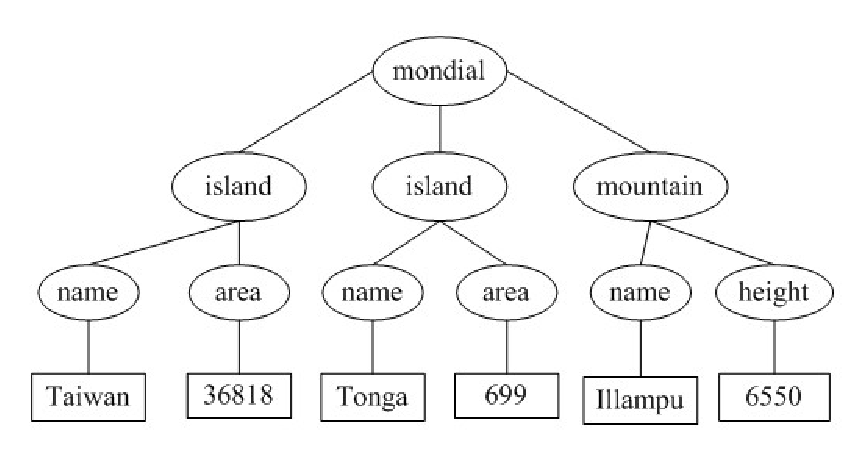
\includegraphics[width=0.4\textwidth]{XML}
\caption{树状结构}\label{fig:xml}
\vspace{\baselineskip}
\end{figure}


其插入图片的代码及其说明如下。
\vspace{1em}\noindent\hrule
\begin{verbatim}
\begin{figure}[htbp]
\centering
\includegraphics[width=0.4\textwidth]{文件名(.eps)}
\caption{标题}\label{标签名(通常为 fig:labelname)}
\vspace{\baselineskip} %表示图与正文空一行
\end{figure}
\end{verbatim}

\noindent\hrule

\begin{verbatim}
figure环境的可选参数[htbp]表示浮动图形所放置的位置,h (here)表示当前位置,t (top)表示页芯顶部,b (bottom)表示页芯底部,p (page)表示单独一页。在Word等软件中,图片通常插入到当前位置,如果当前页的剩余空间不够,图片将被移动到下一页,当前页就会出现很大的空白,其人工调整工作非常不便。由LaTeX提供的浮动图片功能,总是会按h->t->b->p的次序处理选项中的字母,自动调整图片的位置,大大减轻了工作量。
\centering命令将后续内容转换成每行皆居中的格式。
"\includegraphics"的可选参数用来设置图片插入文中的水平宽度,一般表示为正文宽度(\textwidth)的倍数。
\caption命令可选参数“标签名”为英文形式,一般不以图片或表格的数字顺序作为标签,而应包含一定的图片或表格信息,以便于文中引用(若图片、表格、公式、章节和参考文献等在文中出现的先后顺序发生了变化,其标注序号及其文中引用序号也会跟着发生变化,这一点是Word等软件所不能做到的)。另外,图题或表题并不会因为分页而与图片或表格体分置于两页,章节等各级标题也不会置于某页的最底部,LaTeX系统会自动调整它们在正文中的位置,这也是Word等软件所无法匹敌的。
\vspace将产生一定高度的竖直空白,必选参数为负值表示将后续文字位置向上提升,参数值可自行调整。em为长度单位,相当于大写字母M的宽度。\vspace{\baselineskip} 表示图与正文空一行。
引用方法:“见图~\ref{fig:figname}”、“如图~\ref{fig:figname}~所示”等。
\end{verbatim}

\noindent\hrule\vspace{1em}

若需要将~2~张及以上的图片并排插入到一行中,则需要采用\verb|minipage|环境,如图~\ref{fig:dd}~和图~\ref{fig:ds}~所示。
\begin{figure}[htbp]
\centering
\begin{minipage}{0.4\textwidth}
\centering
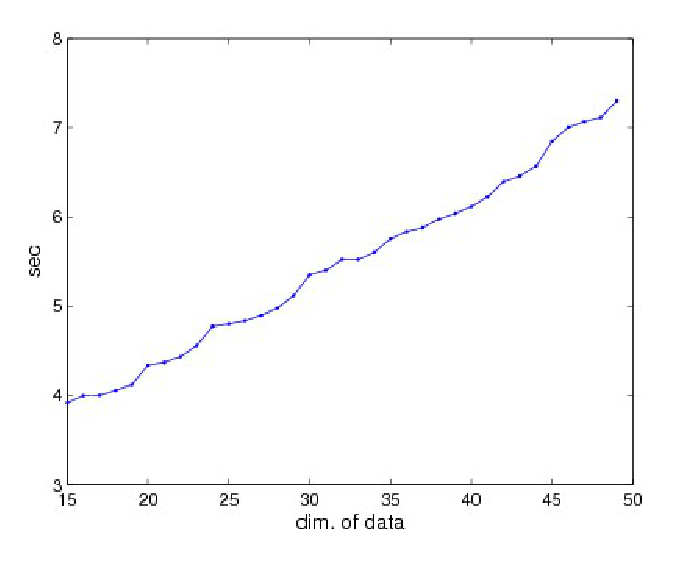
\includegraphics[width=\textwidth]{dataDimensions}
\caption{数据维数的变化}\label{fig:dd}
\end{minipage}
\begin{minipage}{0.4\textwidth}
\centering
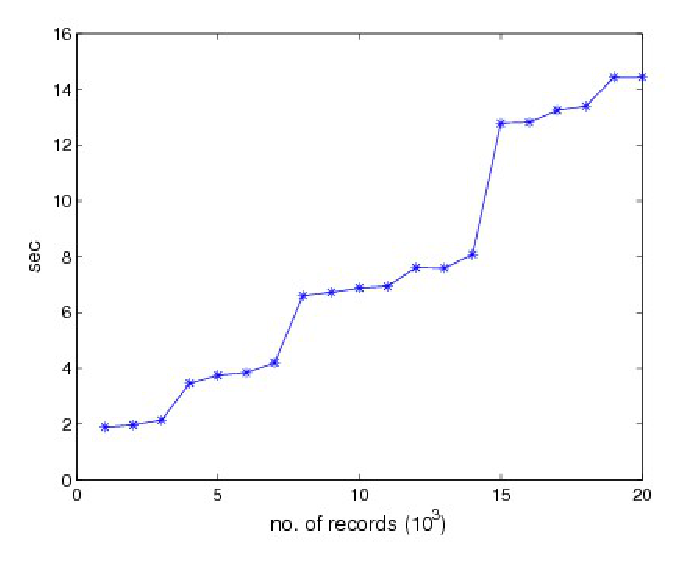
\includegraphics[width=\textwidth]{dataSize}
\caption{数据规模的变化}\label{fig:ds}
\end{minipage}
\vspace{\baselineskip}
\end{figure}

其代码如下所示。
\vspace{1em}\noindent\hrule
\begin{verbatim}
\begin{figure}[htbp]
\centering
\begin{minipage}{0.4\textwidth}
\centering
\includegraphics[width=\textwidth]{文件名}
\caption{标题}\label{fig:f1}
\end{minipage}
\begin{minipage}{0.4\textwidth}
\centering
\includegraphics[width=\textwidth]{文件名}
\caption{标题}\label{fig:f2}
\end{minipage}\vspace{\baselineskip}
\end{figure}
\end{verbatim}

\noindent\hrule

\begin{verbatim}
minipage环境的必选参数用来设置小页的宽度,若需要在一行中插入n个等宽图片,则每个小页的宽度应略小于(1/n)\textwidth。
\end{verbatim}

\noindent\hrule

\section{具有子图的图片插入方法}

图中若含有子图时,需要调用~subfigure~宏包, 如图~\ref{fig:subfig}~所示。
\begin{figure}[htbp]
  \centering
  \subfigure[Data Dimensions]{\label{fig:subfig:datadim}
                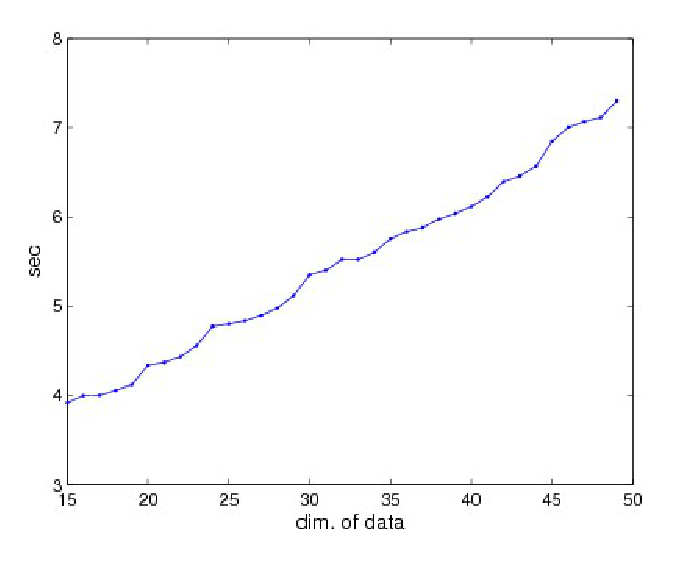
\includegraphics[width=0.4\textwidth]{dataDimensions}}
  \subfigure[Data Size]{\label{fig:subfig:datasize}
                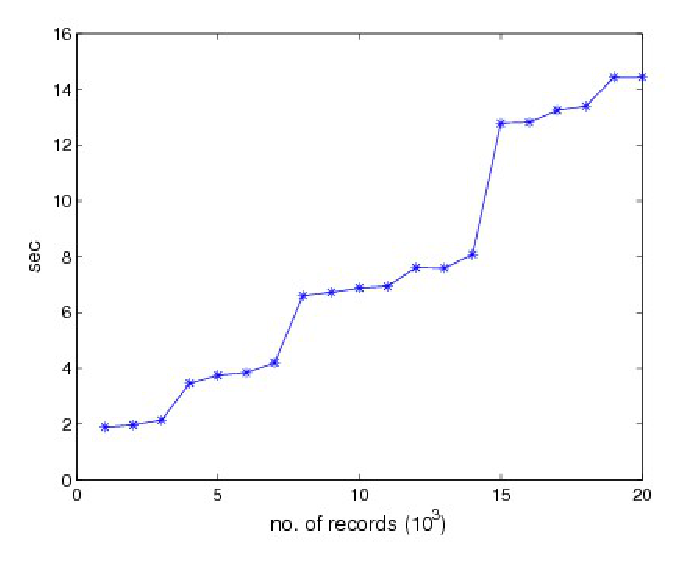
\includegraphics[width=0.4\textwidth]{dataSize}}
  \caption{Scalability of data}\label{fig:subfig}
\vspace{\baselineskip}
\end{figure}

其代码及其说明如下。
\vspace{1em}\noindent\hrule

\begin{verbatim}
\begin{figure}[htbp]
  \centering
  \subfigure[第1个子图标题]{
            \label{第1个子图标签(通常为 fig:subfig1:subsubfig1)}
            \includegraphics[width=0.4\textwidth]{文件名}}
  \subfigure[第2个子图标题]{
            \label{第2个子图标签(通常为 fig:subfig1:subsubfig2)}
            \includegraphics[width=0.4\textwidth]{文件名}}
  \caption{总标题}\label{总标签(通常为 fig:subfig1)}
\vspace{\baselineskip}
\end{figure}
\end{verbatim}

\noindent\hrule

\begin{verbatim}
子图的标签实际上可以随意设定,只要不重复就行。但为了更好的可读性,我们建议fig:subfig:subsubfig格式命名,这样我们从标签名就可以知道这是一个子图引用。
引用方法:总图的引用方法同本章第1节,子图的引用方法用\ref{fig:subfig:subsubfig}来代替。
\end{verbatim}

\noindent\hrule\vspace{1em}

子图的引用示例:如图~\ref{fig:subfig:datadim}~和图~\ref{fig:subfig:datasize}~所示。

若想获得插图方法的更多信息,参见网络上的~\href{ftp://ftp.tex.ac.uk/tex-archive/info/epslatex.pdf}{Using Imported Graphics in \LaTeX and pdf\LaTeX}~文档。 
% !Mode:: "TeX:UTF-8"

\chapter{表格的绘制方法}
\section{研究生毕业设计论文的绘表规范}

表应有自明性。表格不加左、右边线。表的编排建议采用国际通行的三线表。表内中文书写使用宋体五号字。

每个表格之上均应有表题(由表序和表名组成)。表序一般按章编排,如第~1~章第一个插表的序号为“表~1-1”等。表序与表名之间空两格,
表名使用中文五号字,居中。表名中不允许使用标点符号,表名后不加标点。
表头设计应简单明了,尽量不用斜线。表头中可采用化学,物理量等专业符号。

全表如用同一单位,则将单位符号移至表头右上角,加圆括号。
表中数据应准确无误,书写清楚。数字空缺的格内加横线“-”(占~2~个数字宽度)。表内文字或数字上、下或左、右相同时,
采用通栏处理方式,不允许用“〃”、“同上”之类的写法。

表内文字使用宋体五号字,垂直居中书写,起行空一格、转行顶格、句末不加标点。
如某个表需要转页接排,在随后的各页上应重复表的编号。编号后加“(续表)”,表题可省略。续表应重复表头。
表格绘制完成之后,与正文空一行。

\section{普通表格的绘制方法}

表格应具有三线表格式,因此需要调用~booktabs~宏包,其标准格式如表~\ref{tab:table1}~所示。
\begin{table}[htbp]
\caption{符合本科生毕业论文绘图规范的表格}\label{tab:table1}
\vspace{0.5em}\centering\wuhao
\begin{tabular}{ccccc}
\toprule[1.5pt]
$D$(in) & $P_u$(lbs) & $u_u$(in) & $\beta$ & $G_f$(psi.in)\\
\midrule[1pt]
 5 & 269.8 & 0.000674 & 1.79 & 0.04089\\
10 & 421.0 & 0.001035 & 3.59 & 0.04089\\
20 & 640.2 & 0.001565 & 7.18 & 0.04089\\
 5 & 269.8 & 0.000674 & 1.79 & 0.04089\\
10 & 421.0 & 0.001035 & 3.59 & 0.04089\\
20 & 640.2 & 0.001565 & 7.18 & 0.04089\\
 5 & 269.8 & 0.000674 & 1.79 & 0.04089\\
10 & 421.0 & 0.001035 & 3.59 & 0.04089\\
20 & 640.2 & 0.001565 & 7.18 & 0.04089\\
 5 & 269.8 & 0.000674 & 1.79 & 0.04089\\
10 & 421.0 & 0.001035 & 3.59 & 0.04089\\
20 & 640.2 & 0.001565 & 7.18 & 0.04089\\
\bottomrule[1.5pt]
\end{tabular}
\vspace{\baselineskip}
\end{table}

其绘制表格的代码及其说明如下。
\vspace{1em}\noindent\hrule

\begin{verbatim}
\begin{table}[htbp]
\caption{表标题}\label{标签名(通常为 tab:tablename)}
\vspace{0.5em}\centering\wuhao
\begin{tabular}{cc...c}
\toprule[1.5pt]
表头第1个格   & 表头第2个格   & ... & 表头第n个格  \\
\midrule[1pt]
表中数据(1,1) & 表中数据(1,2) & ... & 表中数据(1,n)\\
表中数据(2,1) & 表中数据(2,2) & ... & 表中数据(2,n)\\
表中数据(3,1) & 表中数据(3,2) & ... & 表中数据(3,n)\\
表中数据(4,1) & 表中数据(4,2) & ... & 表中数据(4,n)\\
...................................................\\
表中数据(m,1) & 表中数据(m,2) & ... & 表中数据(m,n)\\
\bottomrule[1.5pt]
\end{tabular}
\vspace{\baselineskip}
\end{table}
\end{verbatim}

\noindent\hrule

\begin{verbatim}
table环境是一个将表格嵌入文本的浮动环境。
\wuhao命令将表格的字号设置为五号字(10.5pt),在绘制表格结束退出时,不需要将字号再改回为\xiaosi,正文字号默认为小四号字(12pt)。
tabular环境的必选参数由每列对应一个格式字符所组成:c表示居中,l表示左对齐,r表示右对齐,其总个数应与表的列数相同。此外,@{文本}可以出现在任意两个上述的列格式之间,其中的文本将被插入每一行的同一位置。表格的各行以\\分隔,同一行的各列则以&分隔。
\toprule、\midrule和\bottomrule三个命令是由booktabs宏包提供的,其中\toprule和\bottomrule分别用来绘制表格的第一条(表格最顶部)和第三条(表格最底部)水平线,\midrule用来绘制第二条(表头之下)水平线,且第一条和第三条水平线的线宽为1.5pt,第二条水平线的线宽为1pt。
引用方法:“如表~\ref{tab:tablename}~所示”。
\end{verbatim}

\noindent\hrule

\section{长表格的绘制方法}

长表格是当表格在当前页排不下而需要转页接排的情况下所采用的一种表格环境。若长表格仍按照普通表格的绘制方法来获得,
其所使用的\verb|table|浮动环境无法实现表格的换页接排功能,表格下方过长部分会排在表格第1页的页脚以下。为了能够实现长表格的转页接排功能,
需要调用~longtable~宏包,由于长表格是跨页的文本内容,因此只需要单独的\verb|longtable|环境,所绘制的长表格的格式如表~\ref{tab:table2}~所示。

此长表格~\ref{tab:table2}~第~2~页的标题“编号(续表)”和表头是通过代码自动添加上去的,无需人工添加,若表格在页面中的竖直位置发生了变化,长表格在第~2~页
及之后各页的标题和表头位置能够始终处于各页的最顶部,也无需人工调整,\LaTeX~系统的这一优点是~Word~等软件所无法企及的。

下段内容是为了让下面的长表格分居两页,看到表标题“编号(续表)”的效果。摘录于《你若安好,便是晴天 -- 林徽因传》片段:

她叫林徽因,出生于杭州,是许多人梦中期待的白莲。她在雨雾之都伦敦,发生过一场空前绝后的康桥之恋。她爱过三个男子,爱得清醒,也爱得平静。徐志摩为她徜徉在康桥,深情地等待一场旧梦可以归来。梁思成与她携手走过千山万水,为完成使命而相约白头。金岳霖为她终身不娶,痴心不改地守候一世。可她懂得人生飘忽不定,要学会随遇而安。
真正的平静,不是避开车马喧嚣,而是在心中修篱种菊。尽管如流往事,每一天都涛声依旧,只要我们消除执念,便可寂静安然。愿每个人在纷呈世相中不会迷失荒径,可以端坐磐石上,醉倒落花前。
如果可以,请让我预支一段如莲的时光,哪怕将来某一天加倍偿还。这个雨季会在何时停歇,无从知晓。但我知道,你若安好,便是晴天。					
\wuhao\begin{longtable}{ccc}
\caption{天津大学各学院名称一览}\label{tab:table2}
 \vspace{0.5em}\\
\toprule[1.5pt] 学院名称 & 网址 & 联系电话  \\ \midrule[1pt]
\endfirsthead
\multicolumn{3}{c}{表~\thetable(续表)}\vspace{0.5em}\\
\toprule[1.5pt] 学院名称 & 网址 & 联系电话  \\ \midrule[1pt]
\endhead
\bottomrule[1.5pt]
\endfoot
机械工程学院& \url{http://tdjxxy.tju.edu.cn/}& 87401979\\
精密仪器与光电子工程学院&  \url{http://www2.tju.edu.cn/colleges/precision/cn/}& 27404775\\
电子信息工程学院& \url{http://www.tju.edu.cn/seie}& 27406956\\
电气与自动化工程学院& \url{http://www2.tju.edu.cn/colleges/automate/}& 27405477\\
建筑工程学院& \url{http://www2.tju.edu.cn/colleges/civil/}& 27404072\\
化工学院& \url{http://chemeng.tju.edu.cn/}& 27403389\\
材料科学与工程学院& \url{http://mse.tju.edu.cn}& 27406693 \\
建筑学院& \url{http://hgw022072.chinaw3.com/}& 27402724-2111\\
求是学部\\
管理与经济学部&	\url{ http://sm.tju.edu.cn}& 27403423\\
理学院& \url{ http://www.tju.edu.cn/science/}& 27404118\\
文法学院& \url{ http://www2.tju.edu.cn/colleges/sociology/new/}& 27403691\\
软件学院& \url{http://scs.tju.edu.cn}& 87401540\\
计算机科学与技术学院& \url{http://cs.tju.edu.cn/}& 27406538\\
马克思主义学院& \url{http://www2.tju.edu.cn/colleges/marxism/}& 27405348\\
环境科学与工程学院& \url{http://www.tju.edu.cn/see}& 87402072\\
药物科学与技术学院& \url{http://www2.tju.edu.cn/colleges/pharmtier/}& 87401830\\
教育学院& \url{http://soe.tju.edu.cn/}& 27401028\\
职业技术教育学院& \url{http://202.113.0.248:8888}\\
继续教育学院& \url{http://aectu.tju.edu.cn/}& 27406298\\
仁爱学院& \url{http://www.tjrac.edu.cn/}& 68579990\\
农业与生物工程学院& \url{http://202.113.13.169/site/nongxueyuan/}& 87402171\\
国际教育学院 & \url{http://www.ietju.com/}& 27406147\\
网络教育学院 & \url{http://www.etju.com/}& 27426952 \\

\end{longtable}\xiaosi
\vspace{\baselineskip}

绘制长表格的代码及其说明如下。
\vspace{1em}\noindent\hrule

\begin{verbatim}
\wuhao\begin{longtable}{cc...c}
\caption{表标题}\label{标签名(通常为 tab:tablename)}\\
\toprule[1.5pt] 表头第1个格 & 表头第2个格 & ... & 表头第n个格\\ \midrule[1pt]
\endfirsthead
\multicolumn{n}{c}{表~\thetable(续表)}\vspace{0.5em}\\
\toprule[1.5pt] 表头第1个格 & 表头第2个格 & ... & 表头第n个格\\ \midrule[1pt]
\endhead
\bottomrule[1.5pt]
\endfoot
表中数据(1,1) & 表中数据(1,2) & ... & 表中数据(1,n)\\
表中数据(2,1) & 表中数据(2,2) & ... & 表中数据(2,n)\\
...................................................\\
表中数据(m,1) & 表中数据(m,2) & ... & 表中数据(m,n)\\
\end{longtable}\xiaosi
\end{verbatim}

\noindent\hrule
\begin{verbatim}
在绘制长表格的前面留出一个空白行,并在第2行的一开始全局定义长表格的字号为五号字,这样能够保证长表格之前段落的行距保持不变。
在绘制长表格结束后,需要\xiaosi命令重新将字号改为小四号字。
\endhead之前的文字描述的是第2页及其之后各页的标题或表头;
\endfirsthead之前的文字描述的是第1页的标题和表头,若无此命令,则第1页的表头和标题由\endhead命令确定;
同理,\endfoot之前的文字描述的是除最后一页之外每页的表格底部内容;
\endlastfoot之前的文字描述的是最后一页的表格底部内容,若无此命令,
则最后一页的表格底部内容由\endfoot命令确定;由于规范中长表格每页底部内容均相同(水平粗线),因此模板中没有用到\endlastfoot命令。
\end{verbatim}

\noindent\hrule
\section{列宽可调表格的绘制方法}
论文中能用到列宽可调表格的情况共有两种:一种是当插入的表格某一单元格内容过长以至于一行放不下的情况,
另一种是当对公式中首次出现的物理量符号进行注释的情况。这两种情况都需要调用~tabularx~宏包。下面将分别对这两种情况下可调表格的绘制方法进行阐述。
\subsection{表格内某单元格内容过长的情况}

首先给出这种情况下的一个例子如表~\ref{tab:table3}~所示。
\begin{table}[htbp]
\caption{最小的三个正整数的英文表示法}\label{tab:table3}
\vspace{0.5em}\wuhao
\begin{tabularx}{\textwidth}{llX}
\toprule[1.5pt]
Value & Name & Alternate names, and names for sets of the given size\\\midrule[1pt]
1 & One & ace, single, singleton, unary, unit, unity\\
2 & Two & binary, brace, couple, couplet, distich, deuce, double, doubleton, duad, duality, duet, duo, dyad, pair, snake eyes, span, twain, twosome, yoke\\
3 & Three & deuce-ace, leash, set, tercet, ternary, ternion, terzetto, threesome, tierce, trey, triad, trine, trinity, trio, triplet, troika, hat-trick\\\bottomrule[1.5pt]
\end{tabularx}
\vspace{\baselineskip}
\end{table}
绘制这种表格的代码及其说明如下。
\vspace{1em}\noindent\hrule
\begin{verbatim}
\begin{table}[htbp]
\caption{表标题}\label{标签名(通常为 tab:tablename)}
\vspace{0.5em}\wuhao
\begin{tabularx}{\textwidth}{l...X...l}
\toprule[1.5pt]
表头第1个格   & ... & 表头第X个格   & ... & 表头第n个格  \\
\midrule[1pt]
表中数据(1,1) & ... & 表中数据(1,X) & ... & 表中数据(1,n)\\
表中数据(2,1) & ... & 表中数据(2,X) & ... & 表中数据(2,n)\\
.........................................................\\
表中数据(m,1) & ... & 表中数据(m,X) & ... & 表中数据(m,n)\\
\bottomrule[1.5pt]
\end{tabularx}
\vspace{\baselineskip}
\end{table}
\end{verbatim}

\noindent\hrule
\begin{verbatim}
tabularx环境共有两个必选参数:第1个参数用来确定表格的总宽度,这里取为排版表格能达到的最大宽度——正文宽度\textwidth;第2个参数用来确定每列格式,其中标为X的项表示该列的宽度可调,其宽度值由表格总宽度确定。
标为X的列一般选为单元格内容过长而无法置于一行的列,这样使得该列内容能够根据表格总宽度自动分行。若列格式中存在不止一个X项,则这些标为X的列的列宽相同,因此,一般不将内容较短的列设为X。
标为X的列均为左对齐,因此其余列一般选为l(左对齐),这样可使得表格美观,但也可以选为c或r。
\end{verbatim}

\noindent\hrule
\subsection{对物理量符号进行注释的情况}
为使得对公式中物理量符号注释的转行与破折号“———”后第一个字对齐,此处最好采用表格环境。此表格无任何线条,左对齐,
且在破折号处对齐,一共有“式中”二字、物理量符号和注释三列,表格的总宽度可选为文本宽度,因此应该采用\verb|tabularx|环境。
由\verb|tabularx|环境生成的对公式中物理量符号进行注释的公式如式(\ref{eq:1})所示。
%\vspace*{10pt}

\begin{equation}\label{eq:1}
\ddot{\boldsymbol{\rho}}-\frac{\mu}{R_{t}^{3}}\left(3\mathbf{R_{t}}\frac{\mathbf{R_{t}\rho}}{R_{t}^{2}}-\boldsymbol{\rho}\right)=\mathbf{a}
\end{equation}

\begin{tabularx}{\textwidth}{@{}l@{\quad}r@{———}X@{}}
式中& $\bm{\rho}$ &追踪飞行器与目标飞行器之间的相对位置矢量;\\
&  $\bm{\ddot{\rho}}$&追踪飞行器与目标飞行器之间的相对加速度;\\
&  $\mathbf{a}$   &推力所产生的加速度;\\
&  $\mathbf{R_t}$ & 目标飞行器在惯性坐标系中的位置矢量;\\
&  $\omega_{t}$ & 目标飞行器的轨道角速度;\\
&  $\mathbf{g}$ & 重力加速度,$=\frac{\mu}{R_{t}^{3}}\left(
3\mathbf{R_{t}}\frac{\mathbf{R_{t}\rho}}{R_{t}^{2}}-\bm{\rho}\right)=\omega_{t}^{2}\frac{R_{t}}{p}\left(
3\mathbf{R_{t}}\frac{\mathbf{R_{t}\rho}}{R_{t}^{2}}-\bm{\rho}\right)$,这里~$p$~是目标飞行器的轨道半通径。
\end{tabularx}
\vspace{\wordsep}

其中生成注释部分的代码及其说明如下。

\vspace{1em}\noindent\hrule

\begin{verbatim}
\begin{tabularx}{\textwidth}{@{}l@{\quad}r@{— — —}X@{}}
式中 & symbol-1 & symbol-1的注释内容;\\
     & symbol-2 & symbol-2的注释内容;\\
     .............................;\\
     & symbol-m & symbol-m的注释内容。
\end{tabularx}\vspace{\wordsep}
\end{verbatim}

\noindent\hrule

\begin{verbatim}
tabularx环境的第1个参数选为正文宽度,第2个参数里面各个符号的意义为:
    第1个@{}表示在“式中”二字左侧不插入任何文本,“式中”二字能够在正文中左对齐,若无此项,则“式中”二字左侧会留出一定的空白;
    @{\quad}表示在“式中”和物理量符号间插入一个空铅宽度的空白;
    @{— — —}实现插入破折号的功能,它由三个1/2的中文破折号构成;
    第2个@{}表示在注释内容靠近正文右边界的地方能够实现右对齐。
\end{verbatim}

\noindent\hrule\vspace{1em}

由此方法生成的注释内容应紧邻待注释公式并置于其下方,因此不能将代码放入\verb|table|浮动环境中。但此方法不能实现自动转页接排,
可能会在当前页剩余空间不够时,全部移动到下一页而导致当前页出现很大空白。因此在需要转页处理时,还请您手动将需要转页的代码放入一个
新的\verb|tabularx|环境中,将原来的一个\verb|tabularx|环境拆分为两个\verb|tabularx|环境。

若想获得绘制表格的更多信息,参见网络上的~\href{http://www.tug.org/pracjourn/2007-1/mori/}{Tables in \LaTeXe: Packages and Methods}~文档。


\include{body/equations}
% !Mode:: "TeX:UTF-8"

\chapter{罗列和定理环境使用方法}

\section{单层罗列环境}
天津大学学位论文一般可采用两种罗列环境:一种是并列条目有同样标签的~\verb|itemize|~罗列环境,另一种是具有自动排序编号符号的~\verb|enumerate|~罗列环境。这两种罗列环境的样式参数可参考图~\ref{fig:list}。
\begin{figure}[htbp]
\centering
\includegraphics[width = 0.6\textwidth]{list}
\caption{罗列环境参数示意图}\label{fig:list}\vspace{-1em}
\end{figure}

通过调用~enumitem~宏包可以很方便地控制罗列环境的布局,其~format.tex~文件中的~\verb|\setitemize|~和~\verb|\setenumerate|~命令分别用来设置~\verb|itemize|~和~\verb|enumerate|~环境的样式参数。采用~\verb|itemize|~单层罗列环境的排版形式如下:

\begin{itemize}
\item 第一个条目文本内容
\item 第二个条目文本内容
\item 第三个条目文本内容
\end{itemize}

其代码如下

\begin{verbatim}
\begin{itemize}
  \item 第一个条目文本内容
  \item 第二个条目文本内容
  ...
  \item 第三个条目文本内容
\end{itemize}
\end{verbatim}

采用~\verb|enumerate|~单层罗列环境的排版形式如下:

\begin{enumerate}
\item 第一个条目文本内容
\item 第二个条目文本内容
\item 第三个条目文本内容
\end{enumerate}

其代码如下

\begin{verbatim}
\begin{enumerate}
  \item 第一个条目文本内容
  \item 第二个条目文本内容
  ...
  \item 第三个条目文本内容
\end{enumerate}
\end{verbatim}



\section{定理环境}

\begin{definition}[谱半径]\label{def:def1}
  称~$n$~阶方阵~$\mathbf{A}$~的全体特征值~$\lambda_1,\cdots,\lambda_n$~组成的集合为~$\mathbf{A}$~的谱,称
  $$\rho(\mathbf{A})=\max{\{|\lambda_1|,\cdots,|\lambda_n|\}}$$
\end{definition}
\begin{theorem}[相似充要条件]\label{lemma:l1}
  方阵$A$和$B$相似的充要条件是:~$A$~和~$B$~有全同的不变因子。
\end{theorem}
\begin{corollary}[推论1]\label{cor:cor1}
在赋范空间~$(X,\|\cdot\|)$~上定义~$d(x,y)=\|x-y\|$, 对任意~$x,y\in X$,~则~$(X,d)$~是距离空间。
\end{corollary}
\begin{proof}
  只需证明~$d(x,y)$~是距离。
\end{proof}
\newpage

定义代码如下:
\begin{verbatim}
 \begin{definition}[谱半径]\label{def:def1}
  称~$n$~阶方阵~$\mathbf{A}$~的全体特征值
  $\lambda_1,\cdots,\lambda_n$组成的集合为~$\mathbf{A}$~的谱,称
  $$\rho(\mathbf{A})=\max{\{|\lambda_1|,\cdots,|\lambda_n|\}}$$
\end{definition}
\end{verbatim}
\noindent\hrule

\vspace{0.1em}\noindent\hrule
\vspace{1em}
定理代码如下:
\begin{verbatim}
\begin{theorem}[相似充要条件]\label{lemma:l1}
  方阵$A$和$B$相似的充要条件是:$A$和$B$有全同的不变因子。
\end{theorem}
\end{verbatim}
\noindent\hrule\vspace{0.1em}

\noindent\hrule
\vspace{1em}
推论和证明代码如下:
\begin{verbatim}
\begin{corollary}[推论1]\label{cor:cor1}
在赋范空间~$(X,\|\cdot\|)$~上定义$d(x,y)=\|x-y\|$,
对任意$x,y\in X$,则$(X,d)$是距离空间。
\end{corollary}
\begin{proof}
  只需证明$d(x,y)$是距离。
\end{proof}
\end{verbatim}
\noindent\hrule\vspace{1em}

定理定义[]中是可选参数,用来说明定理的名称。其他环境格式书写与上面定理、定义、推论格式相同,可自己调用其他环境。
若需要书写定理定义等内容,而且带有顺序编号,需要采用如下环境。除了~\verb|proof|~环境之外,其余~9~个环境都可以有一个可选参数作为附加标题。

\begin{center}
\vspace{0.5em}\noindent\wuhao\begin{tabularx}{0.7\textwidth}{lX|lX}
定理 & \verb|theorem|~环境 & 定义 & \verb|definition|~环境 \\
例 & \verb|example|~环境 & 算法 & \verb|algorithm|~环境 \\
公理 & \verb|axiom|~环境 & 命题 & \verb|proposition|~环境 \\
引理 & \verb|lemma|~环境 & 推论 & \verb|corollary|~环境 \\
注解 & \verb|remark|~环境 & 证明 & \verb|proof|~环境 \\
\end{tabularx}
\end{center} 
\include{body/conclusion}

%%%%%%%%%%  参考文献  %%%%%%%%%%
\defaultfont
\bibliographystyle{TJUThesis}
\phantomsection
\markboth{参考文献}{参考文献}
\addcontentsline{toc}{chapter}{参考文献}       % 参考文献加入到中文目录
\nocite{*}                                     % 若将此命令屏蔽掉,则未引用的文献不会出现在文后的参考文献中
\bibliography{references/reference}
\titleformat{\chapter}{\centering\sihao\hei}{\chaptername}{2em}{}
% !Mode:: "TeX:UTF-8"

\titlecontents{chapter}[2em]{\vspace{.5\baselineskip}\xiaosan\song}%
             {\prechaptername\CJKnumber{\thecontentslabel}\postchaptername\qquad}{} %
             {}             % 设置该选项为空是为了不让目录中显示页码
\addcontentsline{toc}{chapter}{外文资料}
%\setcounter{page}{1}       % 如果需要从该页开始从 1 开始编页,则取消该注释
\markboth{外文资料}{外文资料}
\chapter*{外文资料}

Here follows the English paper.

...              % 外文资料
% !Mode:: "TeX:UTF-8"

\titlecontents{chapter}[2em]{\vspace{.5\baselineskip}\xiaosan\song}
             {\prechaptername\CJKnumber{\thecontentslabel}\postchaptername\qquad}{}
             {}             % 设置该选项为空是为了不让目录中显示页码
\addcontentsline{toc}{chapter}{中文译文}
\setcounter{page}{1}            % 单独从 1 开始编页码
\markboth{中文译文}{中文译文}   % 用于将章节号添加到页眉中
\chapter*{中文译文}

这里就是外文资料的中文翻译。

...
              % 中文译文
\addcontentsline{toc}{chapter}{致\quad 谢} % 添加到目录中
\chapter*{致\quad 谢}

致谢应以简短的文字对课题研究与论文撰写过程中曾直接给予帮助的人员(例如指导教师)表示谢意。“致谢”两字之间空一个全角空格或两个半角空格,采用不编号章标题样式;内容应采用正文样式。
            % 致谢
\clearpage
\end{CJK*}                                     % 结束中文字体使用
\end{document}                                 % 结束全文
